\documentclass[12pt,a4paper]{article}

\usepackage[margin=0.75in]{geometry}
\usepackage{xcolor}
\usepackage{amsmath,amssymb}
\usepackage{booktabs}
\usepackage{tabularx}
\usepackage{tcolorbox}
\usepackage{listings}
\usepackage{helvet}                  
\usepackage[scaled=1.10]{inconsolata} 
\usepackage{graphicx}
\usepackage{subcaption}
\usepackage{float}
\usepackage{tikz}
\usepackage{hyperref}
\usetikzlibrary{positioning, arrows.meta, calc}

\hypersetup{
    colorlinks=true,
    urlcolor=blue
}

\title{Mobile Charger}
\author{
  \textbf{Arjun R Iyengar} \\
  \small ee26btech11202\\
  \and
  \textbf{Arya Sudhirkumar Neel} \\
  \small ee26btech11203\\ \\}
\date{September 2026}
\begin{document}
\maketitle
\section*{Day 1}
\noindent{We spent this day to understand the circuit, its components, function of each component. We got a basic idea of how the charger will look.}
\section*{Day 2}
\noindent{We started by attempting to solder a wire onto the transformer as shown in the picture below. This proved to be challenging as this was our first time soldering. It nearly took $5$ minutes to solder the first wire. We also realised that the soldering rod was not heating properly as the tip of the rod was completely blackened. We had to change the solder before continuing.}

\begin{figure}[H]
    \centering

    \begin{subfigure}[H]{0.45\textwidth}
    \centering
        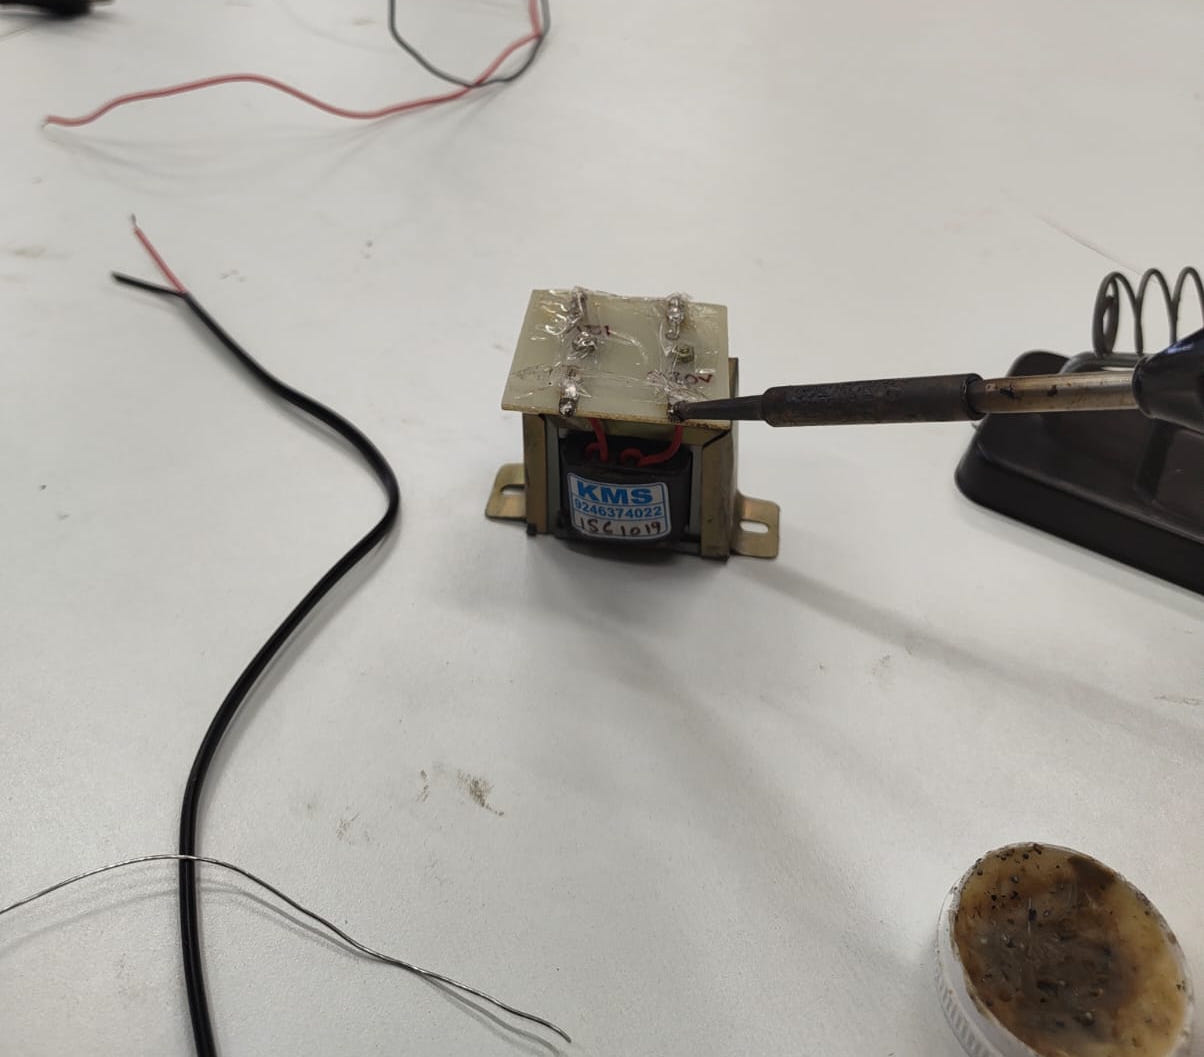
\includegraphics[width=\textwidth, height=8cm, keepaspectratio]{figs/First_solder.jpeg}
        \caption{Front view}
    \end{subfigure}
    \hfill
    \begin{subfigure}[H]{0.45\textwidth}
    \centering
        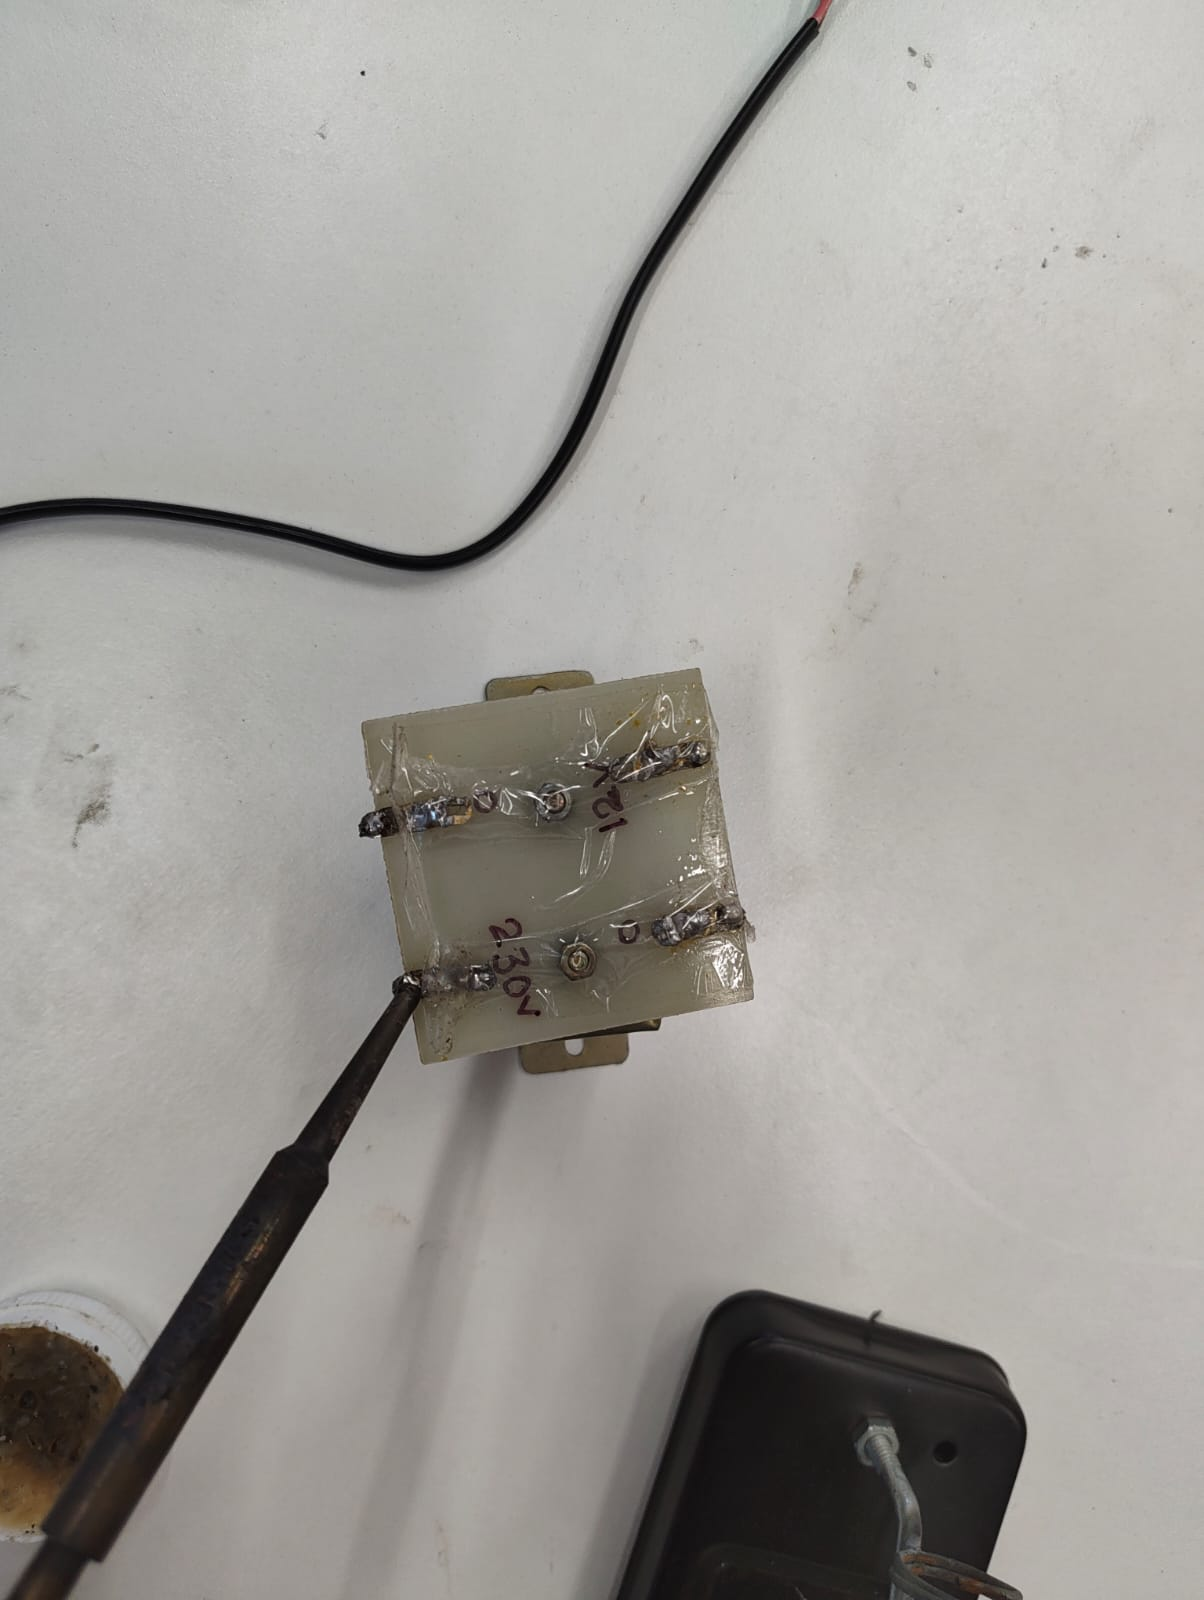
\includegraphics[width=\textwidth, height=8cm, keepaspectratio]{figs/First_solder_top.jpeg}
        \caption{Top view}
    \end{subfigure}


\end{figure}

\noindent{We then finished the soldering for the second wire and the two wires of the plug, improving our soldering technique in the process. Each of us took a turn in soldering. This was the progress after finishing $3$ solders and finishing the final solder.}

\begin{figure}[H]
\centering
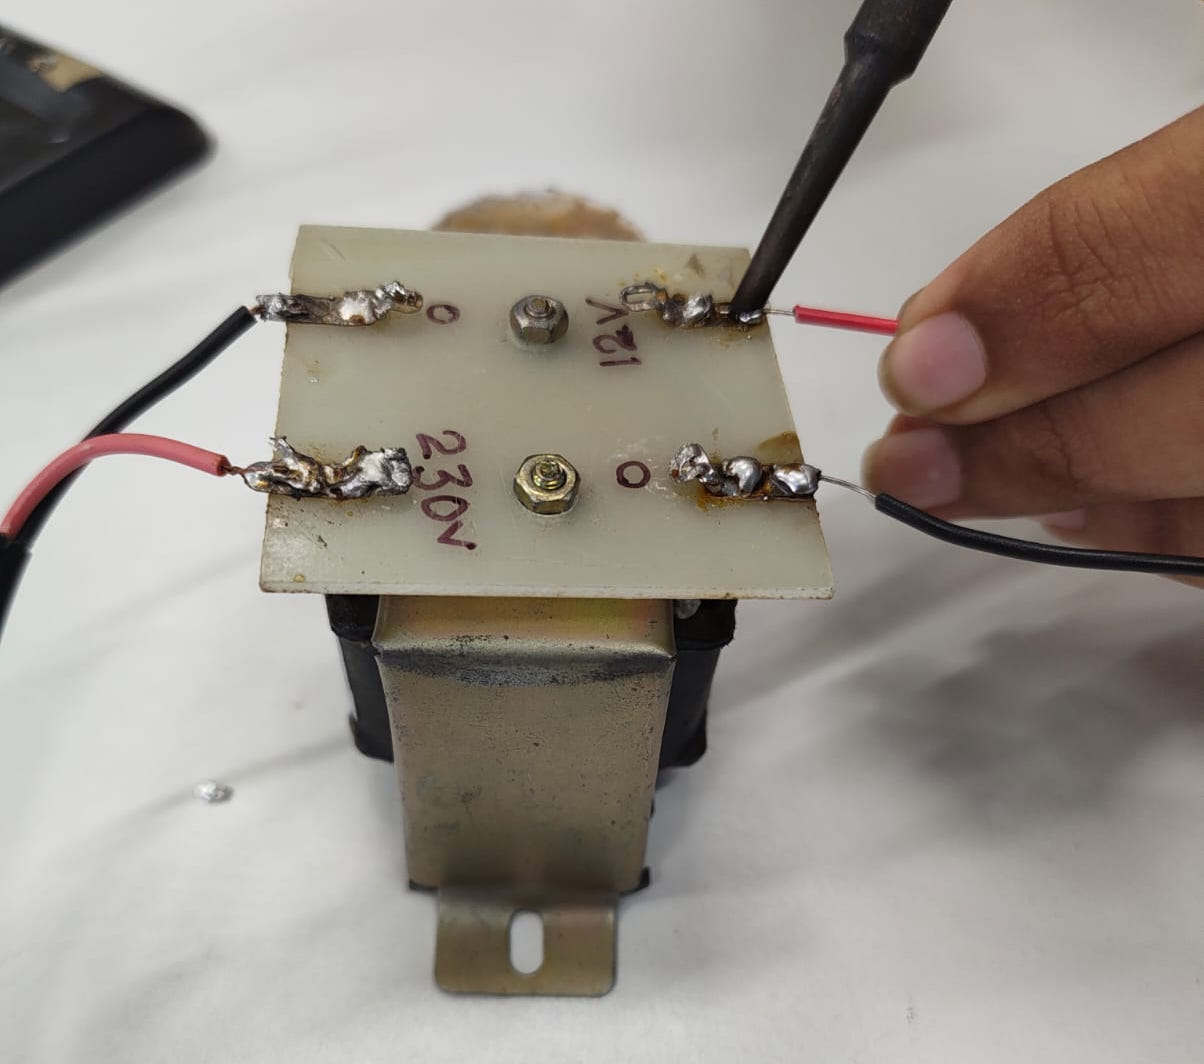
\includegraphics[width=0.60\textwidth]{figs/Soldering_1.jpeg}

\end{figure}
\noindent{We followed this by taking the multimeter readings to check if the transformer is functioning correctly. The following figure shows the AC voltage and frequency readings.}
\begin{figure}[H]
    \centering

    \begin{subfigure}{0.45\textwidth}
    \centering
        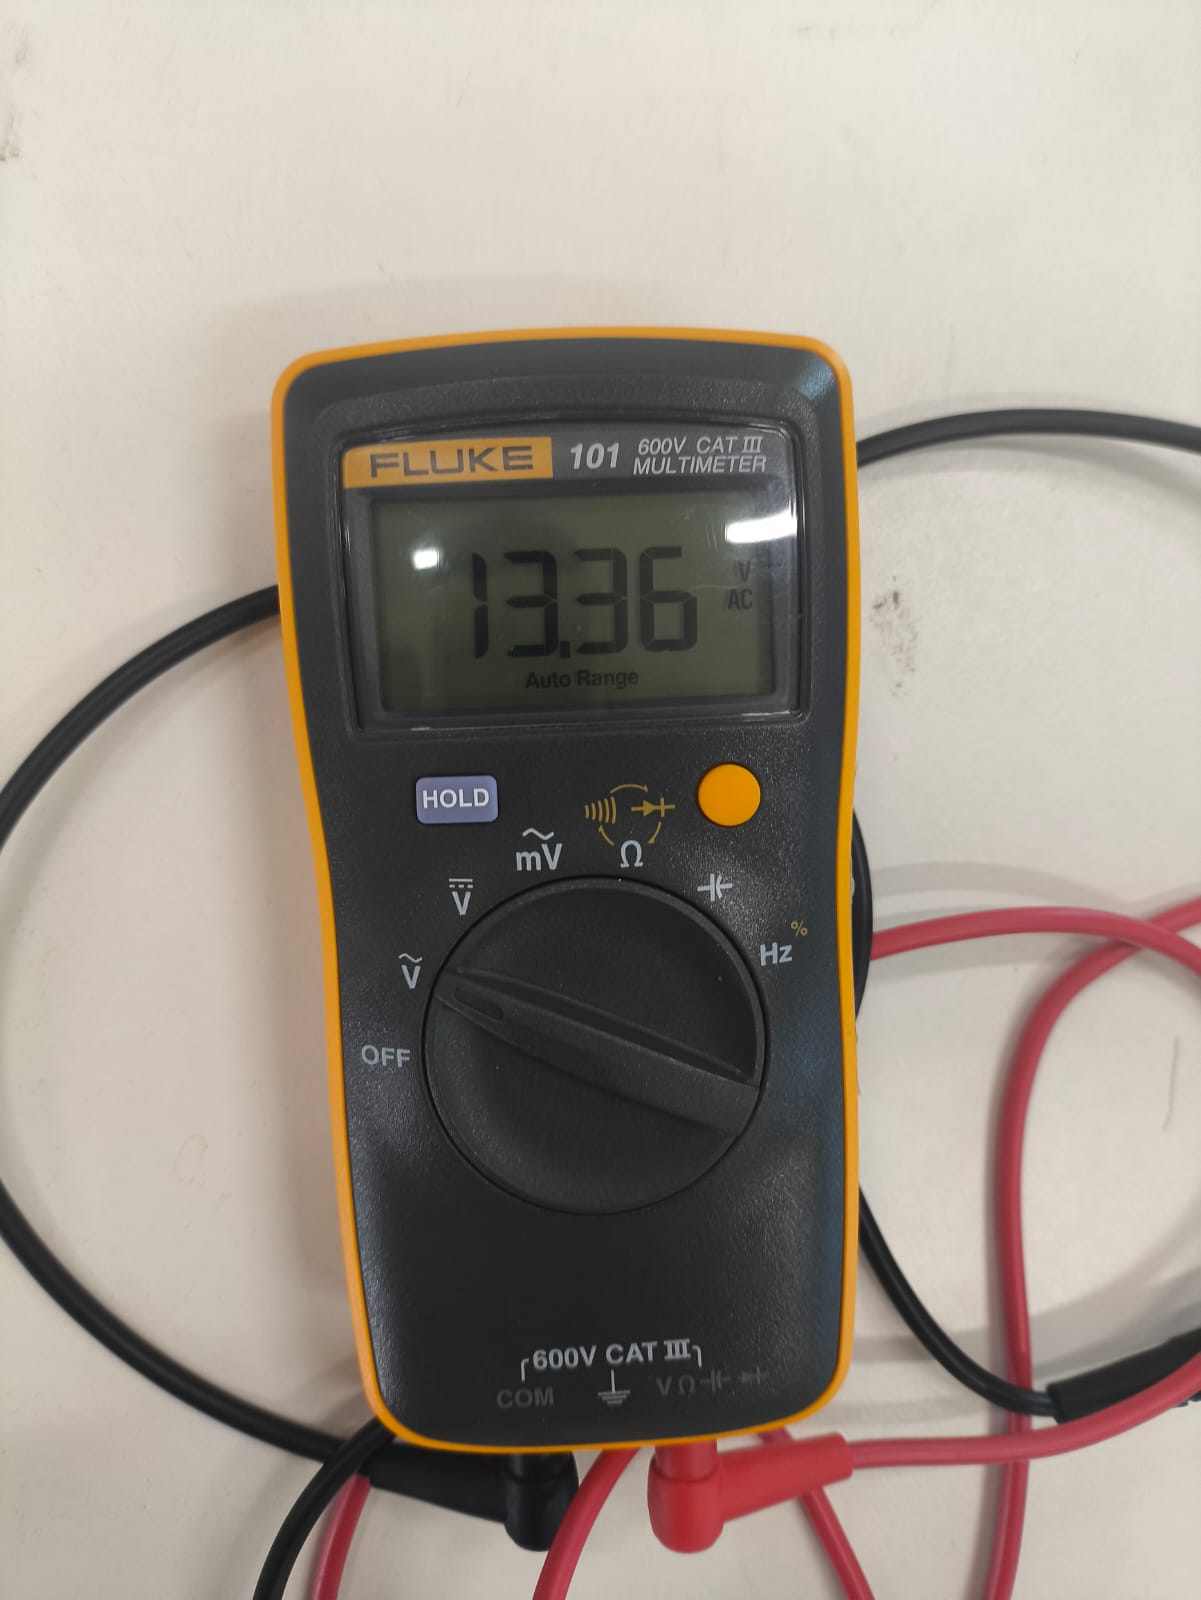
\includegraphics[width=\textwidth, height=10cm, keepaspectratio]{figs/Multimeter_1.jpeg}
        \caption{AC voltage}
    \end{subfigure}
    \hfill
    \begin{subfigure}{0.45\textwidth}
    \centering
        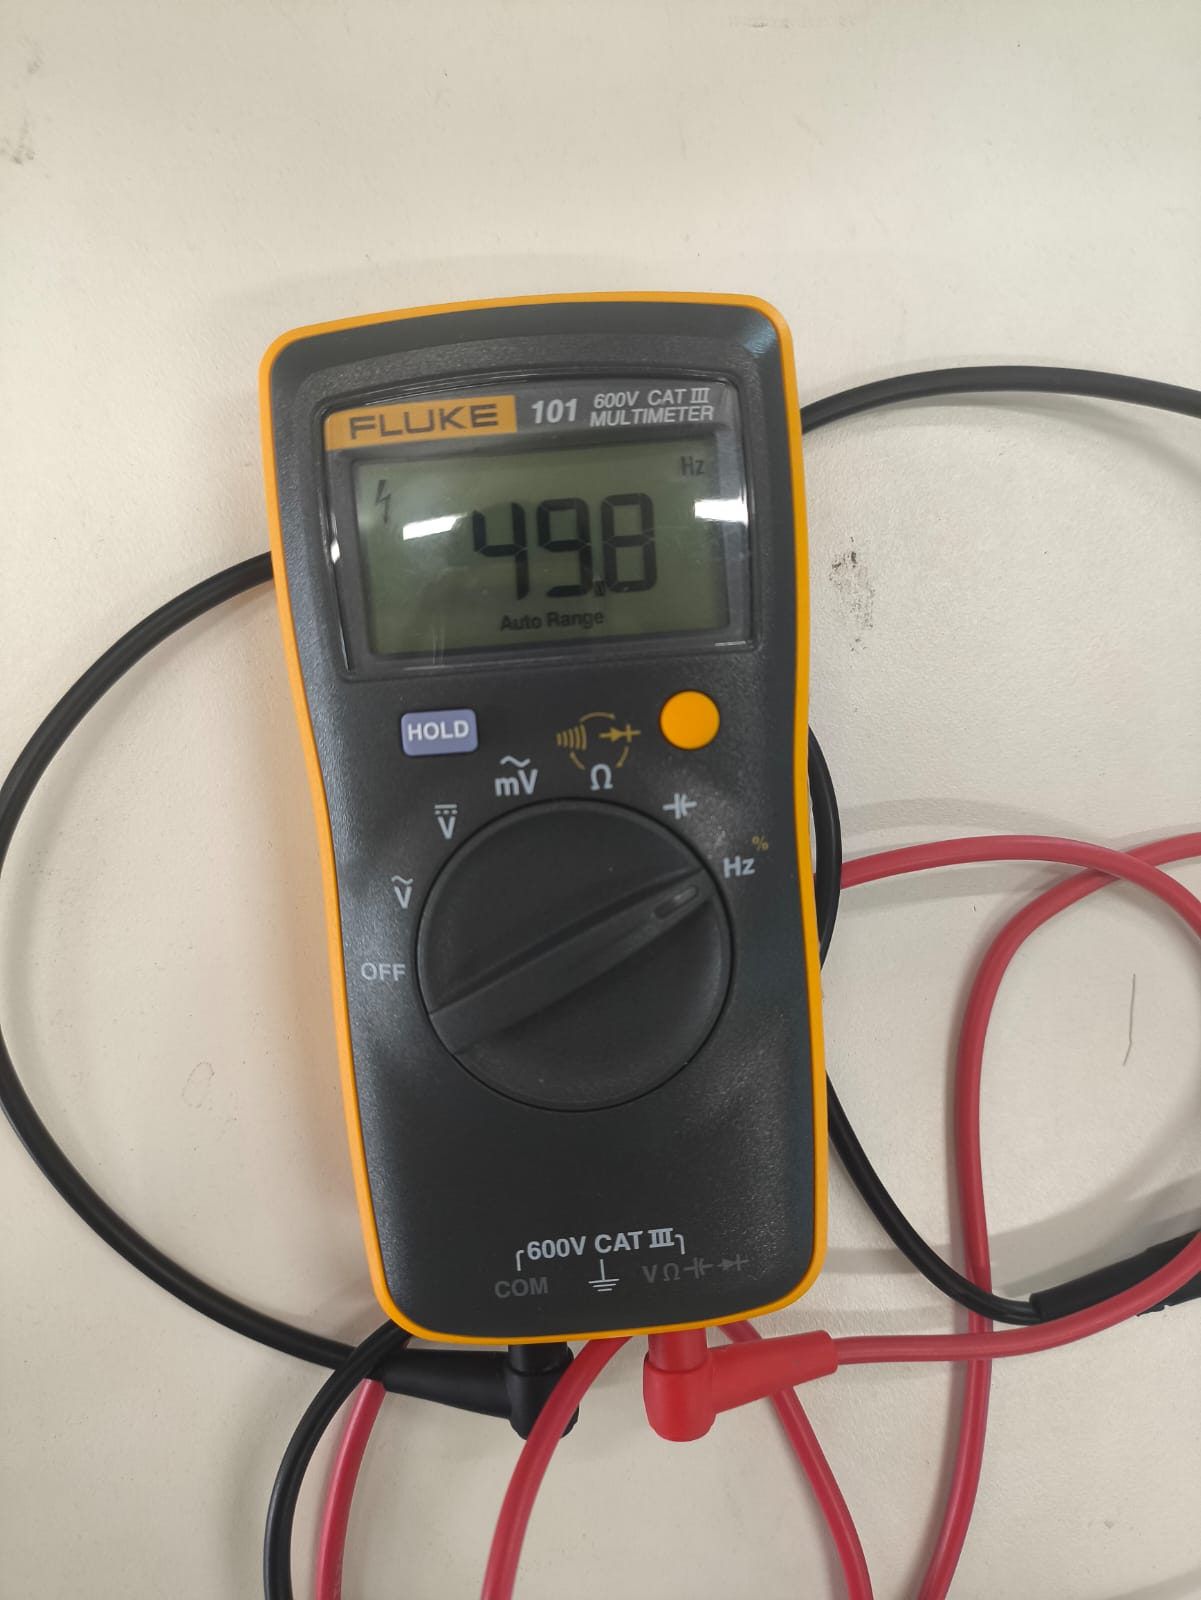
\includegraphics[width=\textwidth, height=10cm, keepaspectratio]{figs/Multimeter_1_freq.jpeg}
        \caption{Frequency}
    \end{subfigure}


\end{figure}
\noindent{We then started working on the circuit, first by placing the diodes to form a bridge rectifier as shown, to get an idea about spacing and  how the circuit will begin to look.}
\begin{figure}[H]
\centering
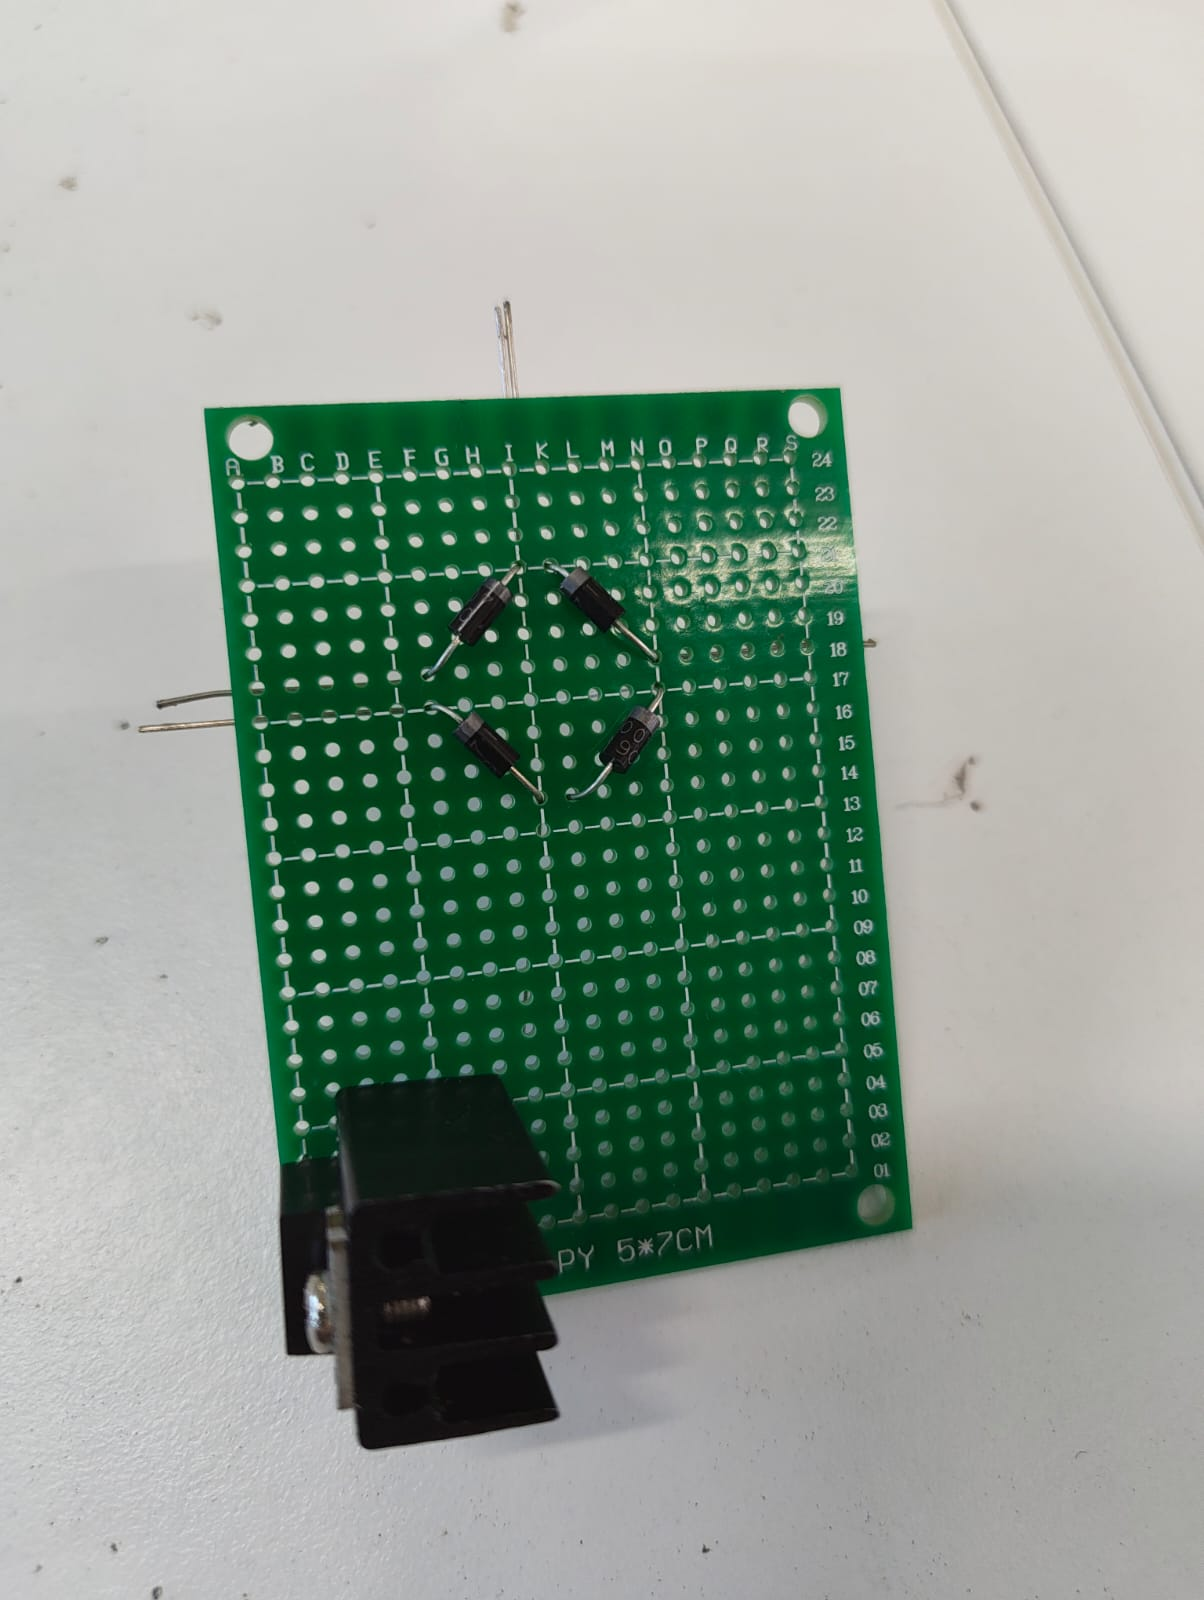
\includegraphics[width=0.60\textwidth]{figs/Bridge_rectifier.jpeg}
\end{figure}
\noindent{This was the initial idea for how the circuit will look:}
\begin{figure}[H]
\centering
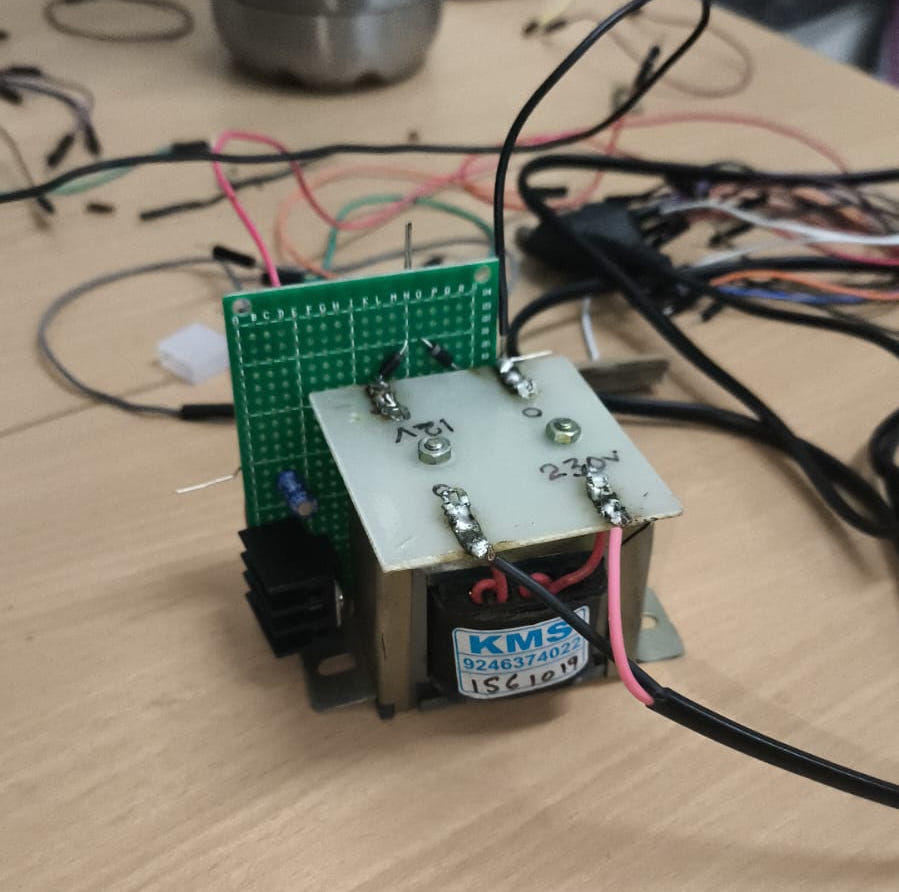
\includegraphics[width=\textwidth, height=10cm, keepaspectratio]{figs/Initial_idea.jpeg}
\end{figure}
\noindent{We then soldered the diodes in place and took the multimeter readings across the DC output, as shown in the figure below.  }
\begin{figure}[H]
\centering
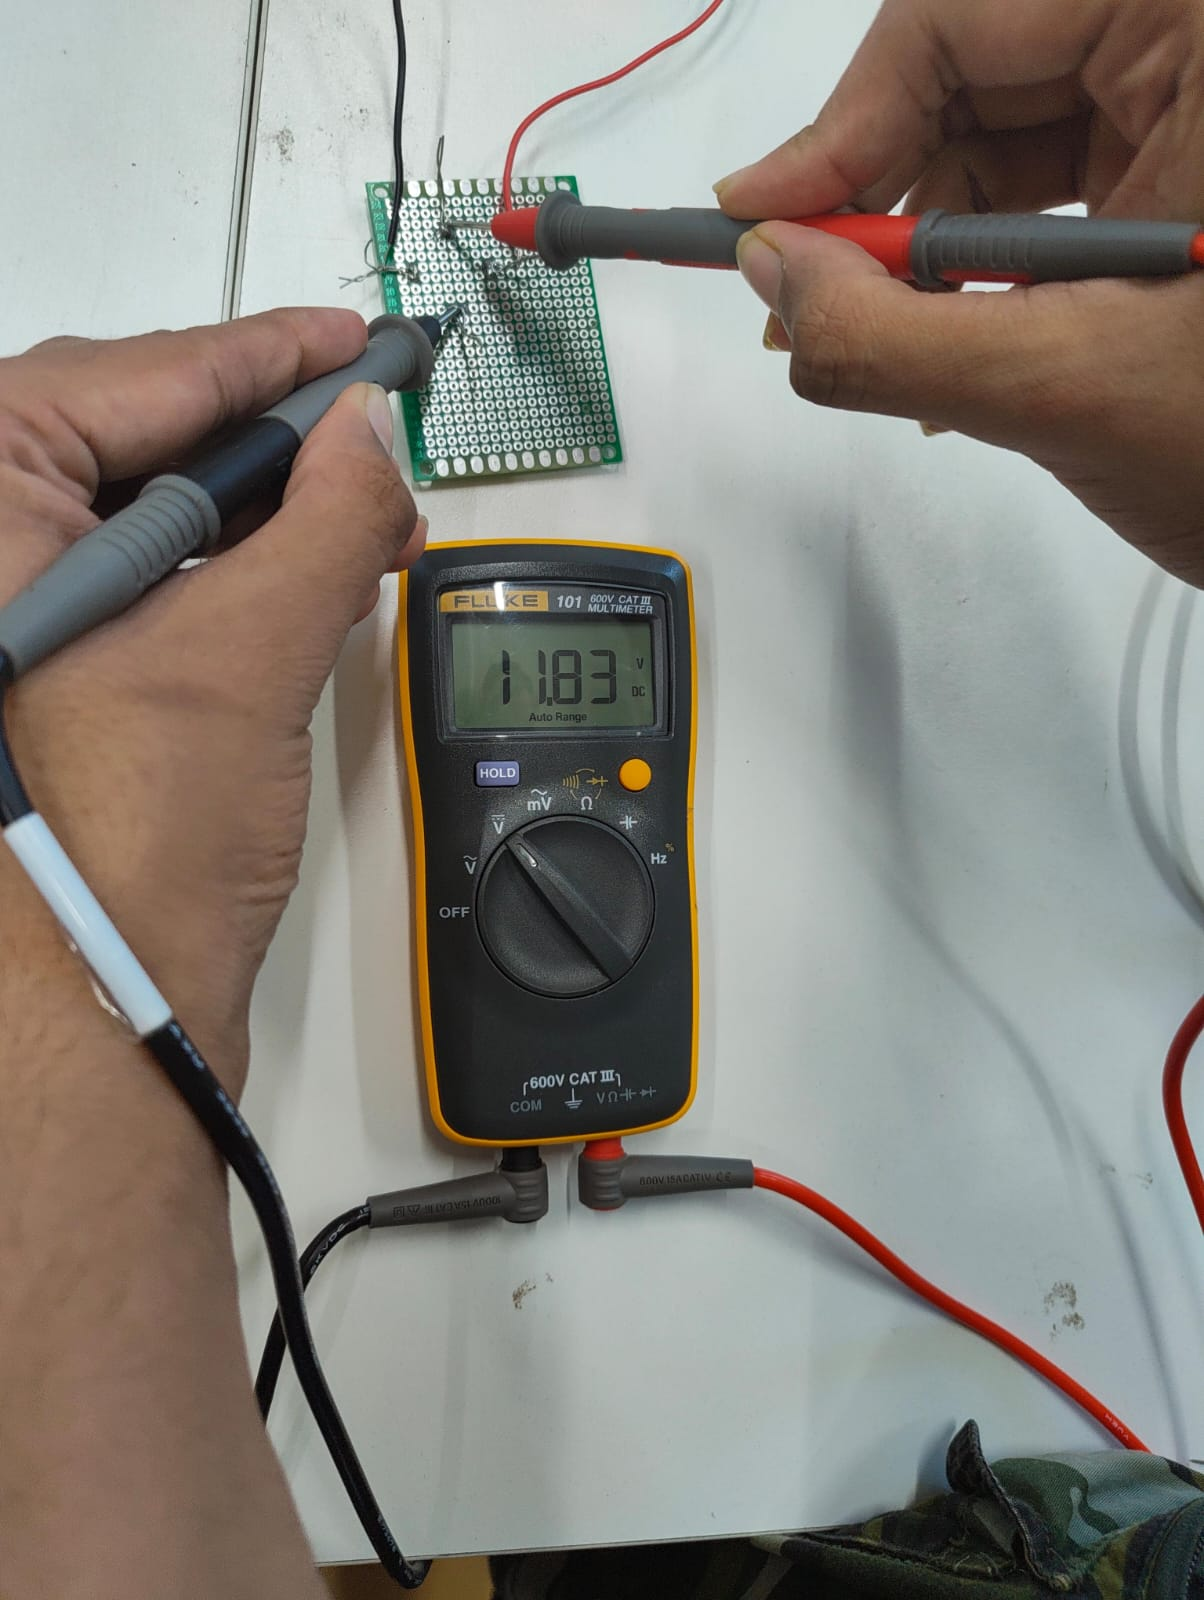
\includegraphics[width=\textwidth, height=10cm, keepaspectratio]{figs/Multimeter_2_DC.jpeg}
\end{figure}

\noindent{We then soldered the capacitor and the input pin of the 7805 regulator, ending our work for the day, as shown in in the following figure.}

\begin{figure}[H]
\centering
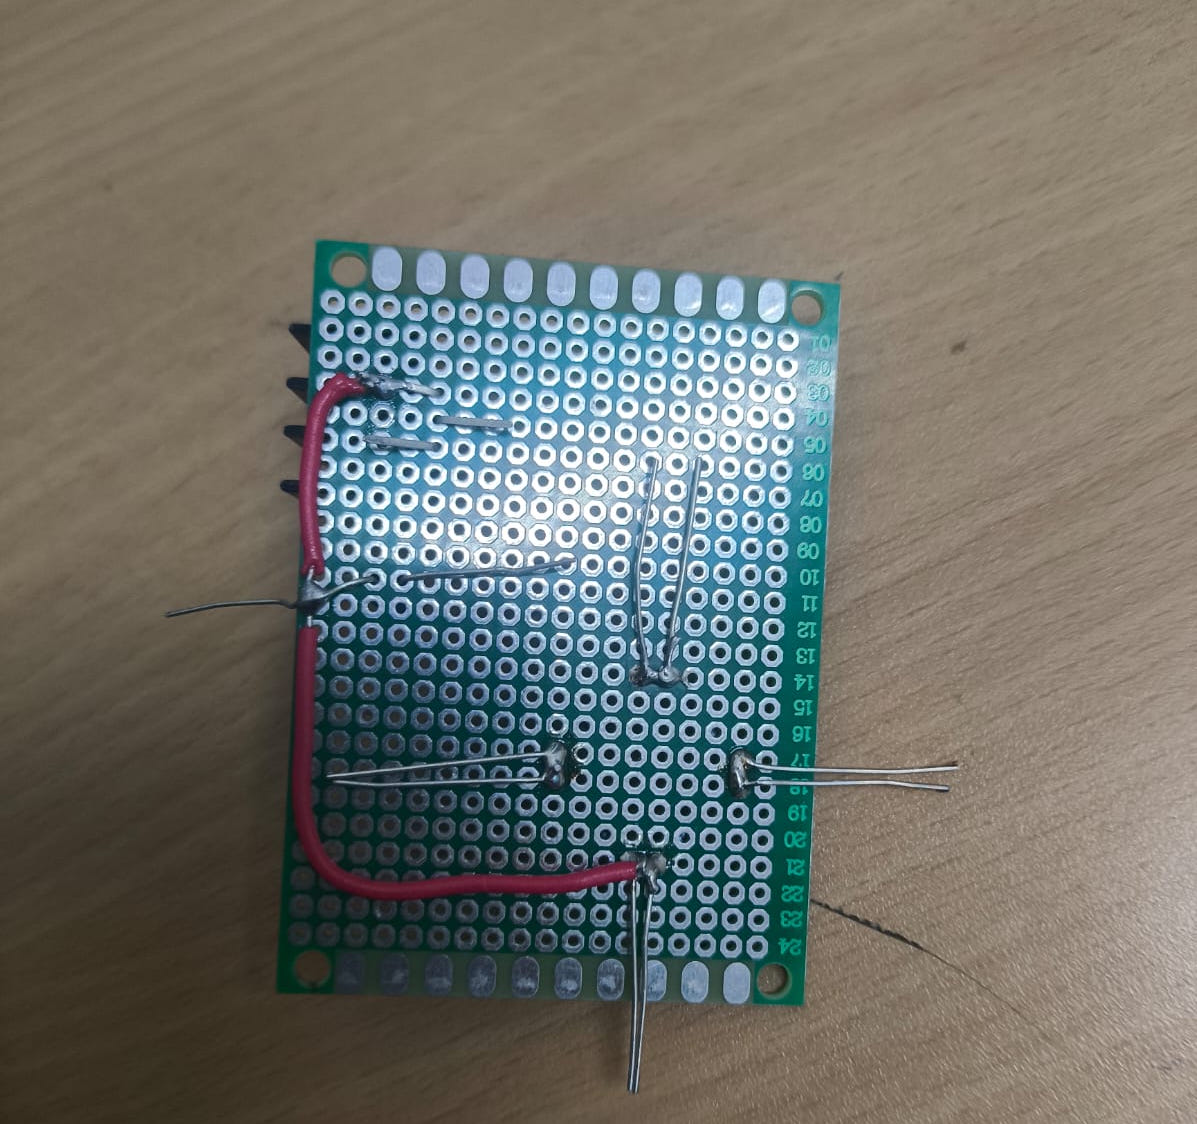
\includegraphics[width=\textwidth, height=10cm, keepaspectratio]{figs/Soldering_2.jpeg}
\end{figure}
\noindent{However, we were disapointed when we found out that the soldering we had done was not great. We had not brought boxes to carry the transformer, and since we took the transformer in our bags, 3 of the wires got detached. We soldered it again trying to improve our technique.}
\section*{Day 3}
\noindent{We realised that the regulator and the capacitor are placed too close in our circuit, as the regulator's heat sink heats up very quickly, and that we had to de-solder and re-solder to improve the spacing for these components. We spent most of the day redoing the circuit. This was the final soldered circuit: }

\begin{figure}[H]
    \centering
    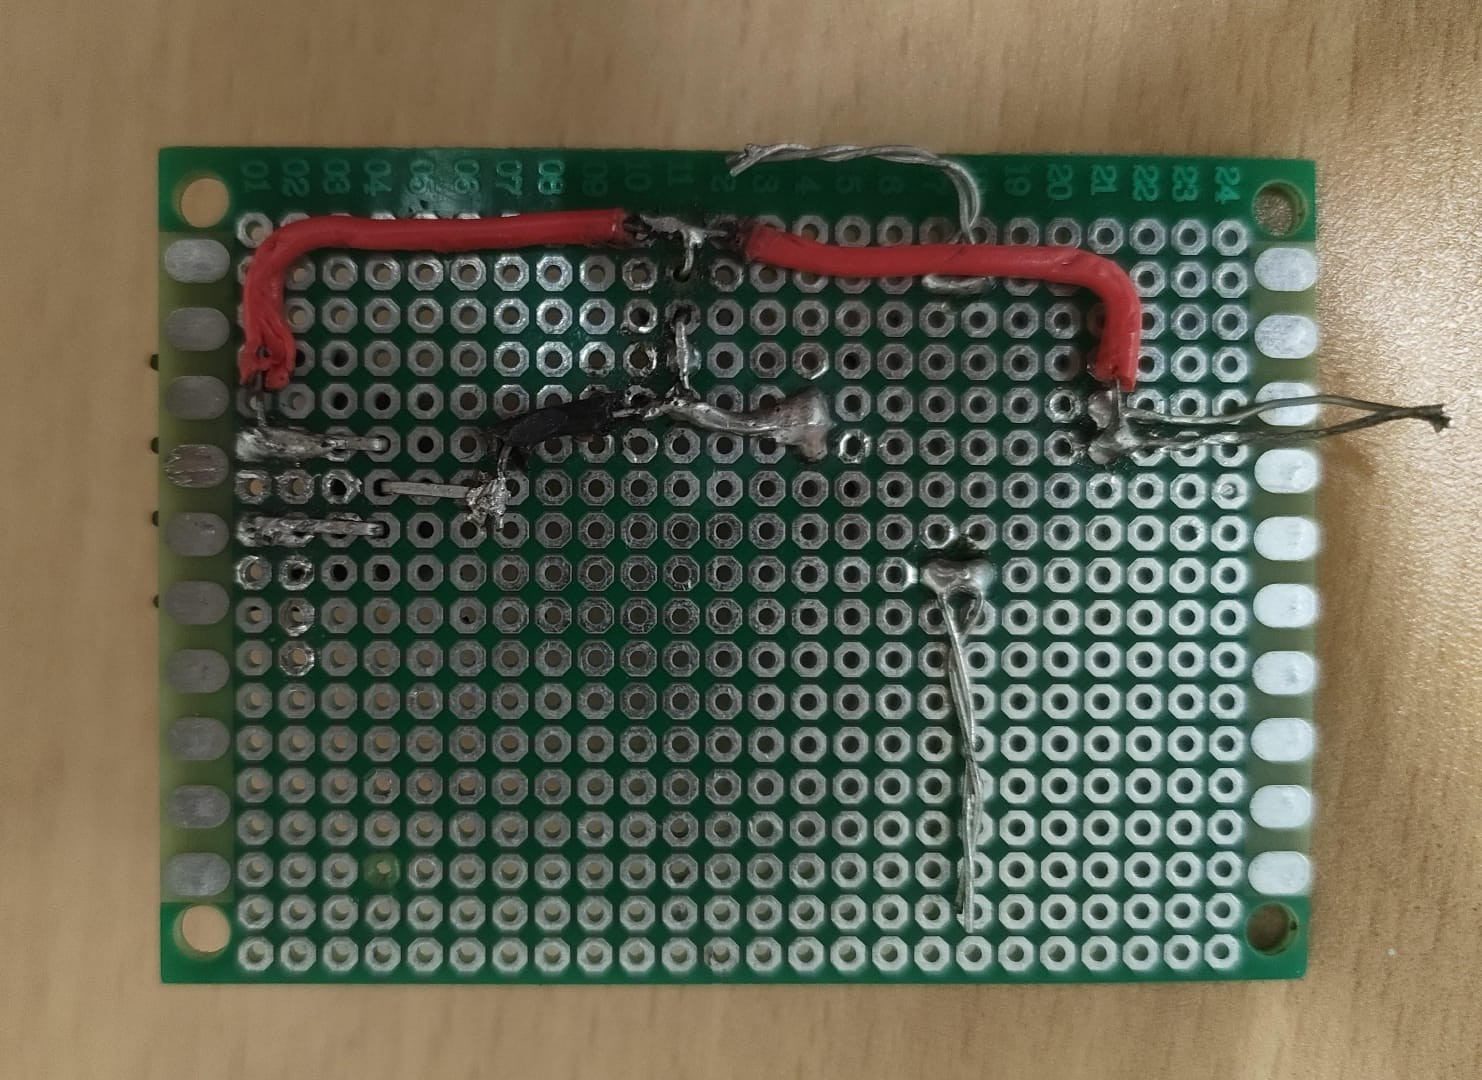
\includegraphics[width=\textwidth, height=10cm, keepaspectratio]{figs/Soldering_3.jpeg}

\end{figure}

\noindent{The spacing on the circuit looked like this: }
\begin{figure}[H]
    \centering
    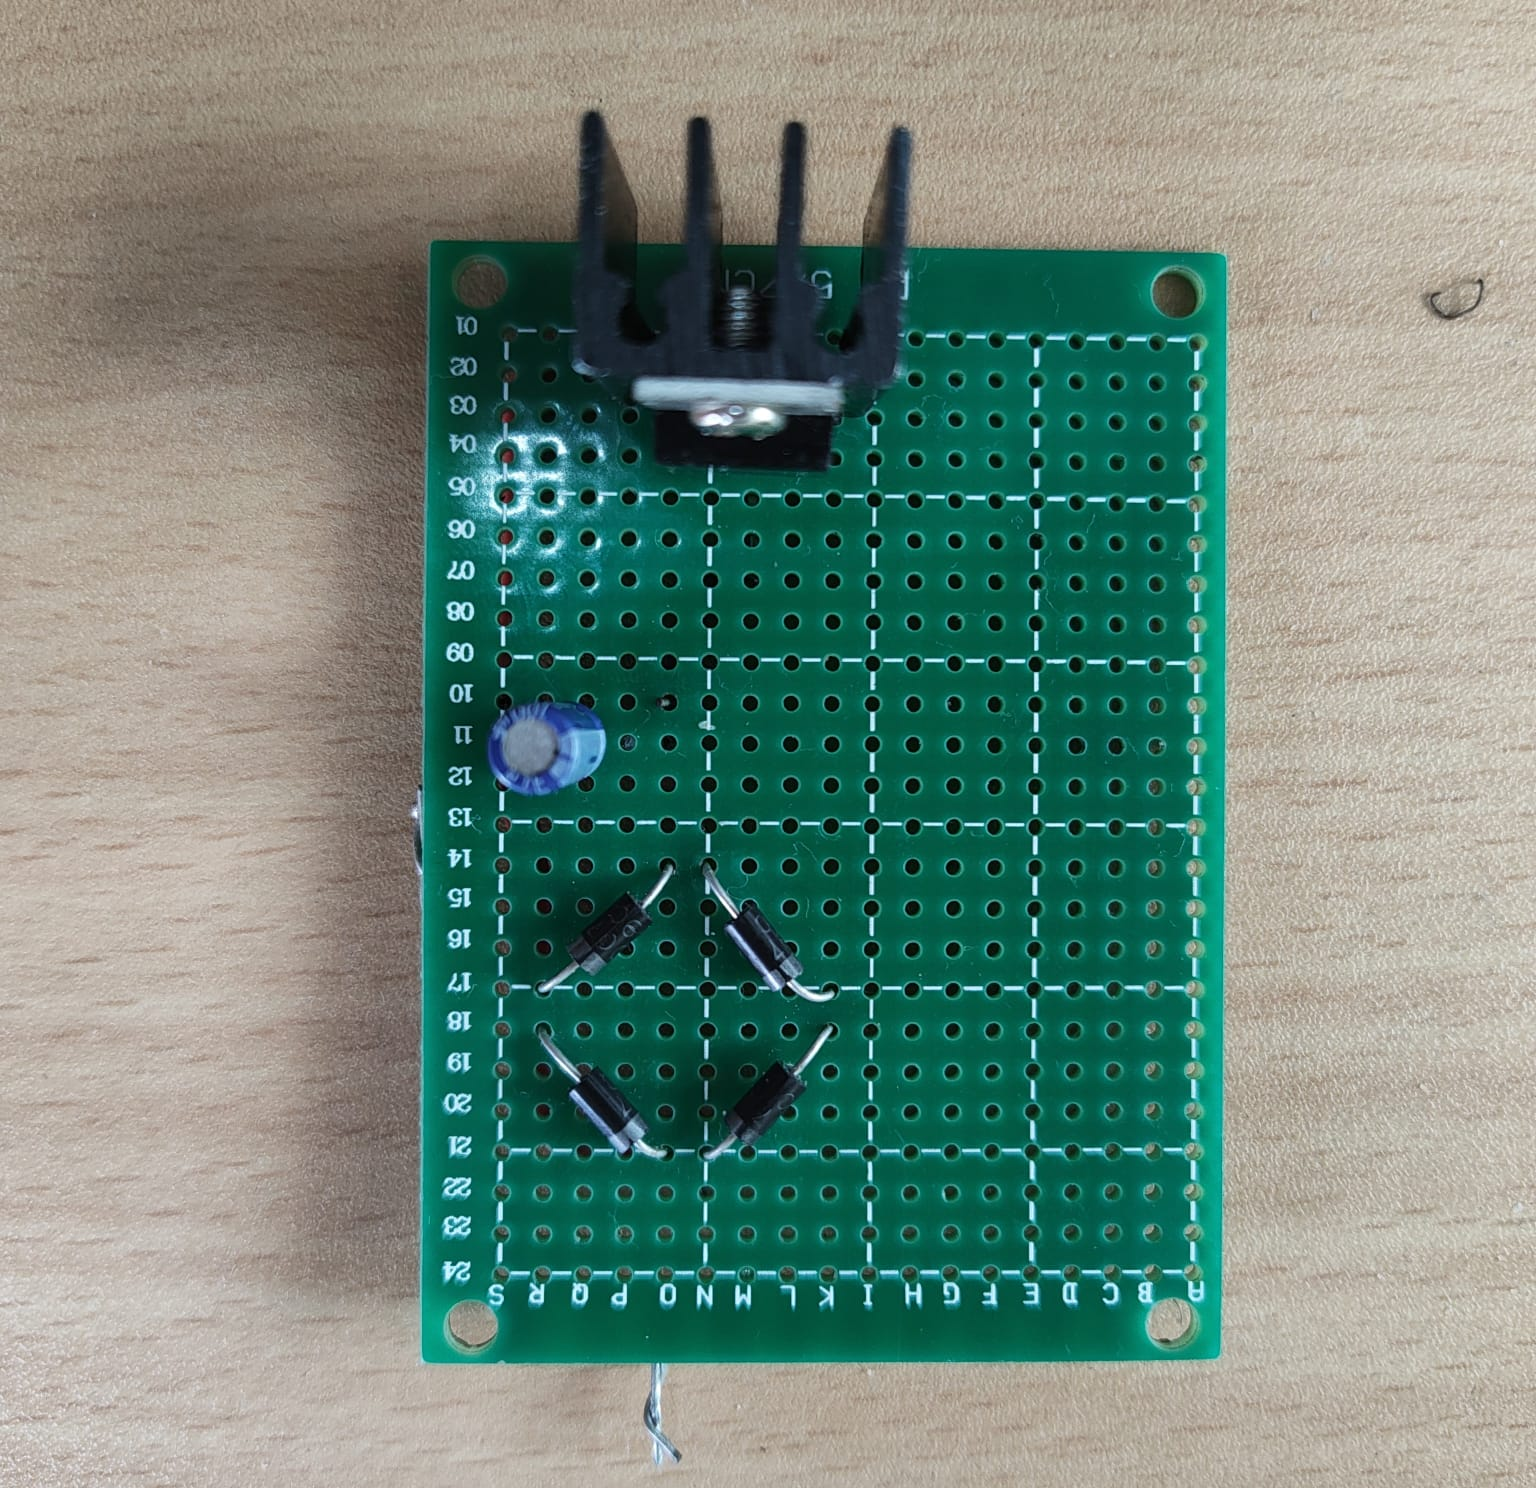
\includegraphics[width=\textwidth, height=10cm, keepaspectratio]{figs/Spaced_circuit.jpeg}
    
\end{figure}

\noindent{Upon soldering them, we took the multimeter readings for the DC voltage across the capacitor, and between the regulator's output and the ground. The following figure shows the multimeter readings: }
\begin{figure}[H]
    \centering

    \begin{subfigure}{0.45\textwidth}
    \centering
        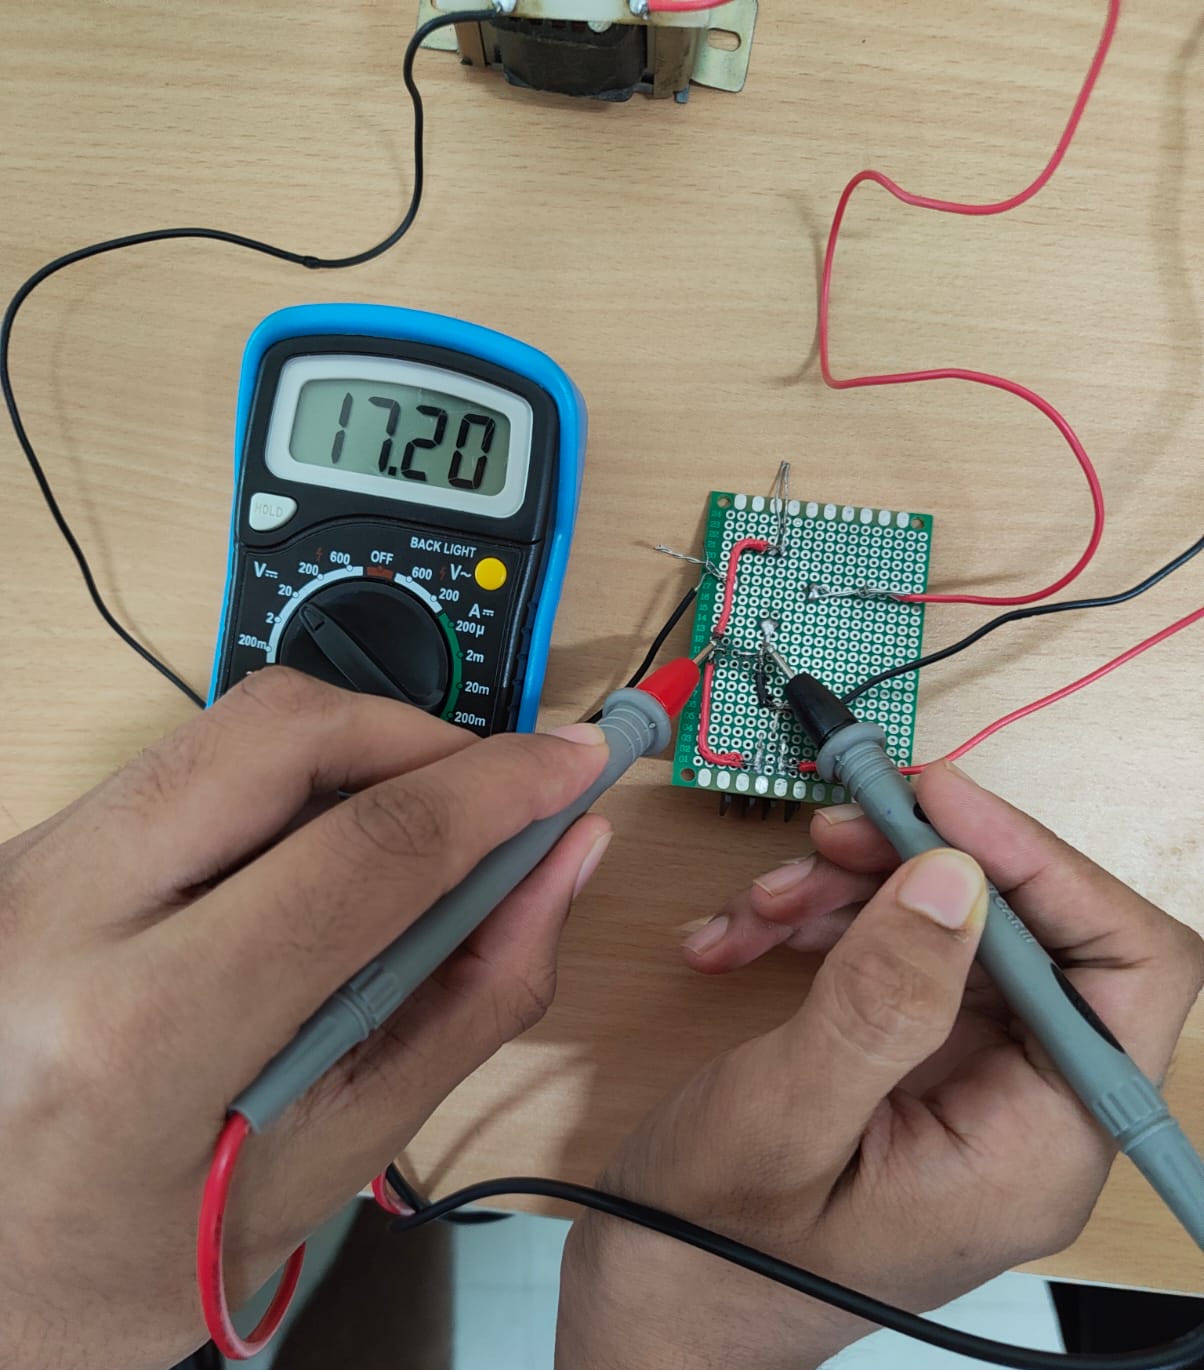
\includegraphics[width=\textwidth, height=10cm, keepaspectratio]{figs/Multimeter_3.jpeg}
        \caption{Voltage across capacitor}
    \end{subfigure}
    \hfill
    \begin{subfigure}{0.45\textwidth}
    \centering
        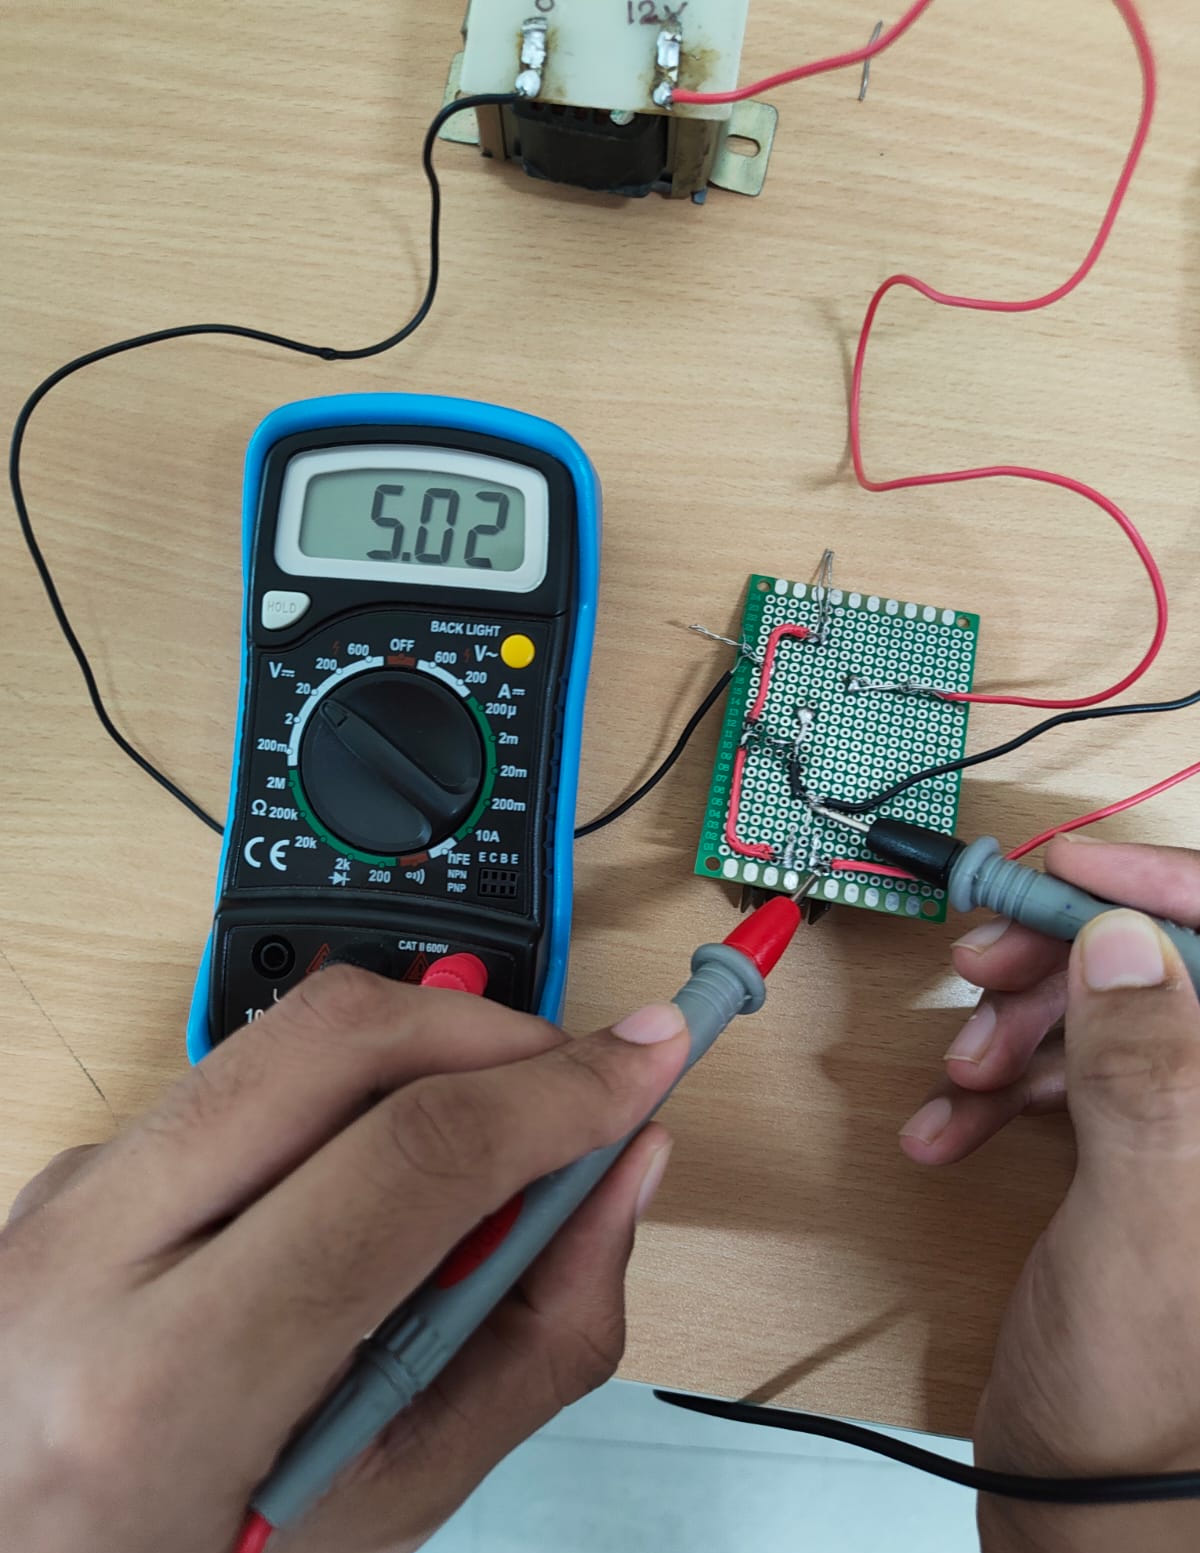
\includegraphics[width=\textwidth, height=9cm, keepaspectratio]{figs/Multimeter_4.jpeg}
        \caption{Voltage output from regulator}
    \end{subfigure}

\end{figure}
\noindent{We followed this by polishing the solders by de-soldering and re-soldering, so that they look better visually.} \\ \\

\noindent{Now that we knew that the charger gave an output of $5V$ via the multimeter, we wanted to check if it actually worked or not. For this, we temporarily connected the ground pin and output pin of the regulator to the respective USB port pins, and used a USB-C cable to charge the phone. This finished the work for the day. The following video shows the  working of this basic charger.} 

\begin{center}
\url{https://youtube.com/shorts/34qiqDtbMtI?feature=share}
\end{center}
\section*{Days 4, 5 and 6}
\noindent{We spent these days trying to learn FreeCAD in order to design the model. We learnt the basic operations like pad, revolve, groove etc. We learnt about implementing constraints, offsets etc.}


\section*{Day 7}
\noindent{The major issue that we faced while brainstorming about the model was how the case would be closed. Upon researching, we found a few methods of doing this, but using a sliding lid was what we decided to go for. These are some other methods we found and why we rejected them: } 
\begin{itemize}
    \item Use of snap joints- We found that this would not work with PLA, and the material would break quickly
    \item Use of screws or pegs- This is not a very reusable option, and also we would have to design the screws separately.
\end{itemize}
\noindent{The idea we came up with was to split the case into two compartments, with a gap in between for the wires, to have a support with slits for the perfboard, and a few supports for the transformer as well. We also planned a compartment for the USB port on the case, instead of soldering it onto the circuit. We took the appropriate measurements required to sketch the model}

\noindent{The starting of the model was quite hard, as we were unsure which approach and where to start from. Eventually we got the idea to begin by sketching a rectangle, filleting its edges and creating an offset. After creating the sketch, we used the pad operation to add volume. Here is the result: }
\begin{figure}[H]
\centering
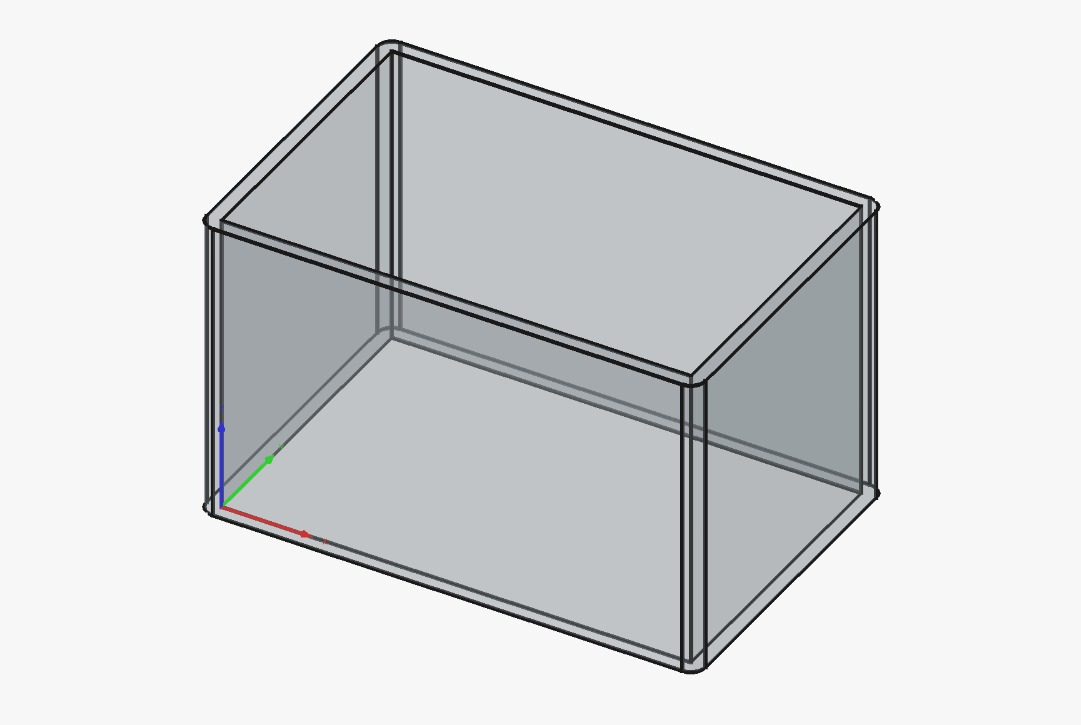
\includegraphics[width=\textwidth, height=10cm, keepaspectratio]{figs/CAD_1.jpeg}
\end{figure}
\noindent{Now with this approach, the base was missing, so we had to add that as well, so we created a new sketch and made the rounded rectangular base, and padded it again.}
\begin{figure}[H]
    \centering
    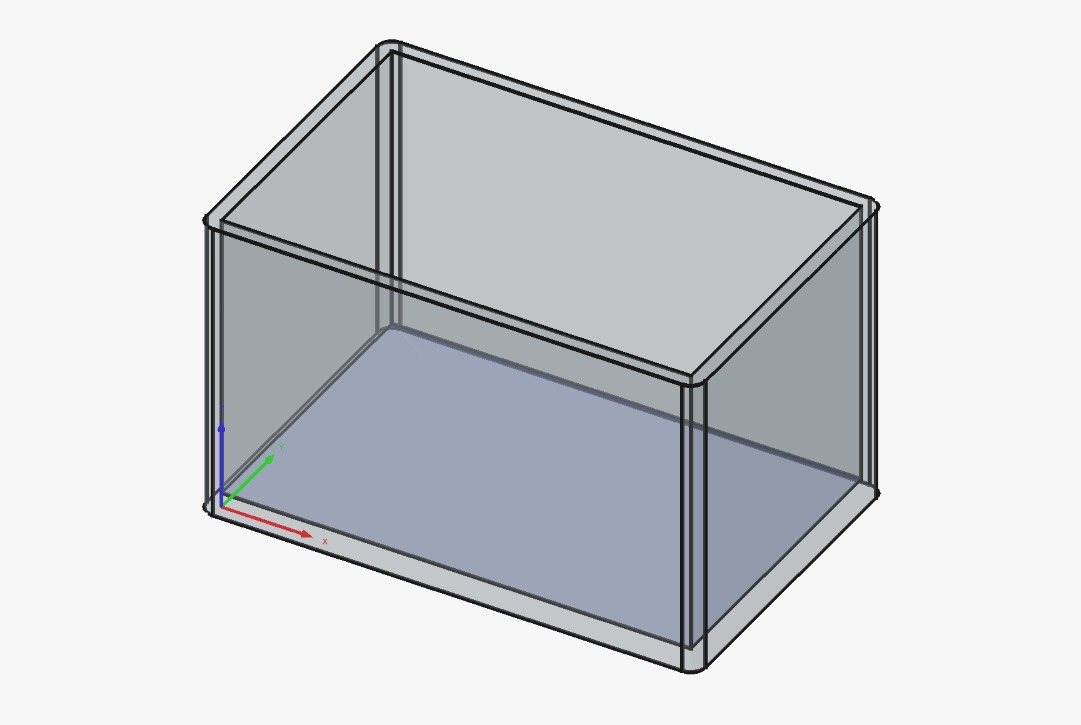
\includegraphics[width=\textwidth, height=10cm, keepaspectratio]{figs/CAD_2.jpeg}

\end{figure}

\noindent{Next, we added the sketch of the separator which creates a space for the transformer. The gap between them is for the ease of movement of wires connecting the transformer to the rectifier. The following figure has the initial sketch before padding.}
\begin{figure}[H]
\centering
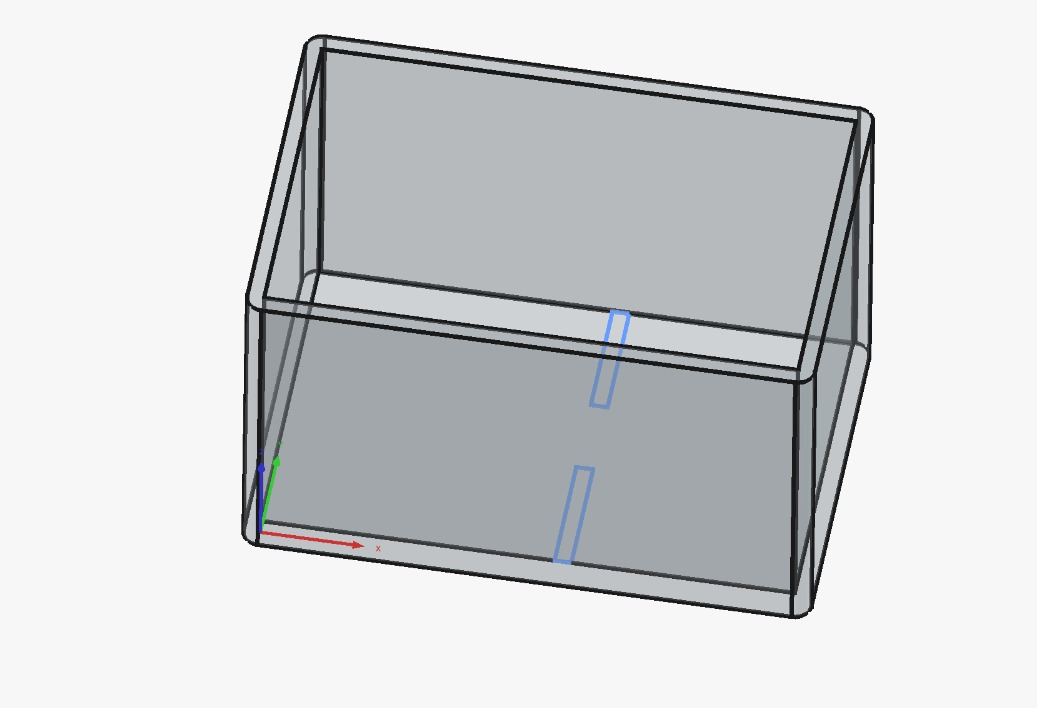
\includegraphics[width=\textwidth, height=11cm, keepaspectratio]{figs/CAD_3.jpeg}
\end{figure}
\noindent{Upon padding, the model looked like this:}
\begin{figure}[H]
\centering
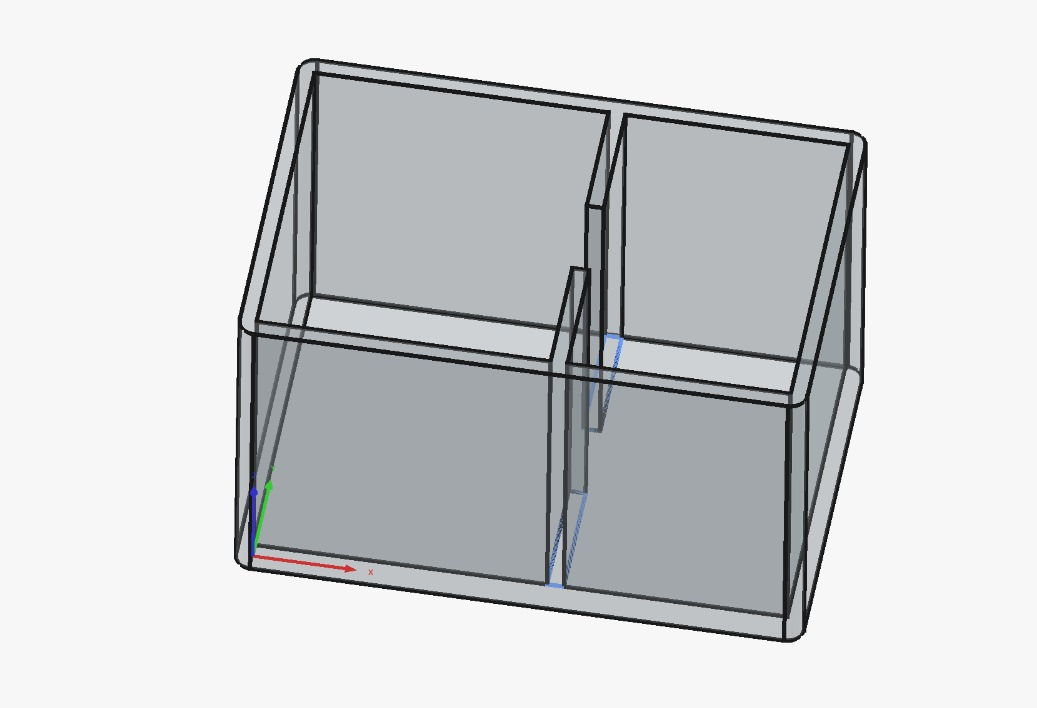
\includegraphics[width=\textwidth, height=11cm, keepaspectratio]{figs/CAD_4.jpeg}
\end{figure}

\noindent{Next, we added a similar structure, but this time with two slits for the perfboard to be supported.}
\begin{figure}[H]
\centering
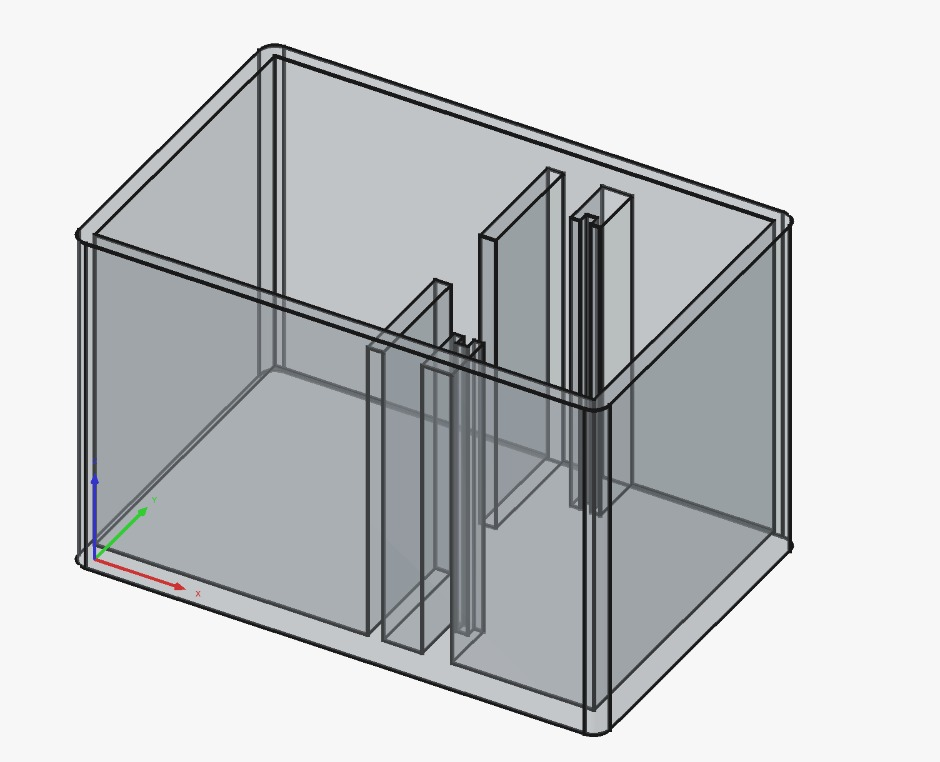
\includegraphics[width=\textwidth, height=11cm, keepaspectratio]{figs/CAD_5.jpeg}
\end{figure}
\noindent{Now, we wanted to add the compartment/pocket for the USB port, but we were unsure in what way we wanted the wires from the regulator to go to the USB port. One option was directly from above the perfboard, however, we didn't want the wires to interfere with regulator, so we decided to create a pocket on the side to facilitate the connection. This also would help by supporting the wires.} \\ \\
\noindent{This was the sketch for the pocket: }
\begin{figure}[H]
\centering
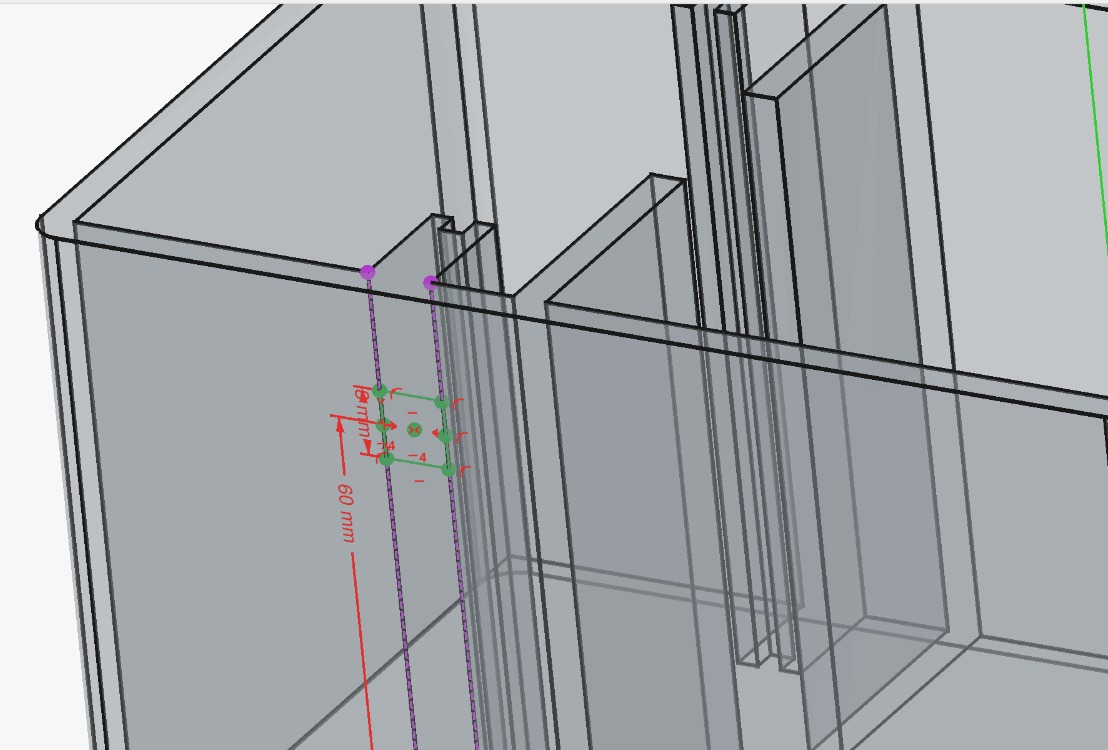
\includegraphics[width=\textwidth, height=9cm, keepaspectratio]{figs/CAD_6.jpeg}
\end{figure}
\noindent{Upon adding volume, the pocket looked like this: }
\begin{figure}[H]
\centering
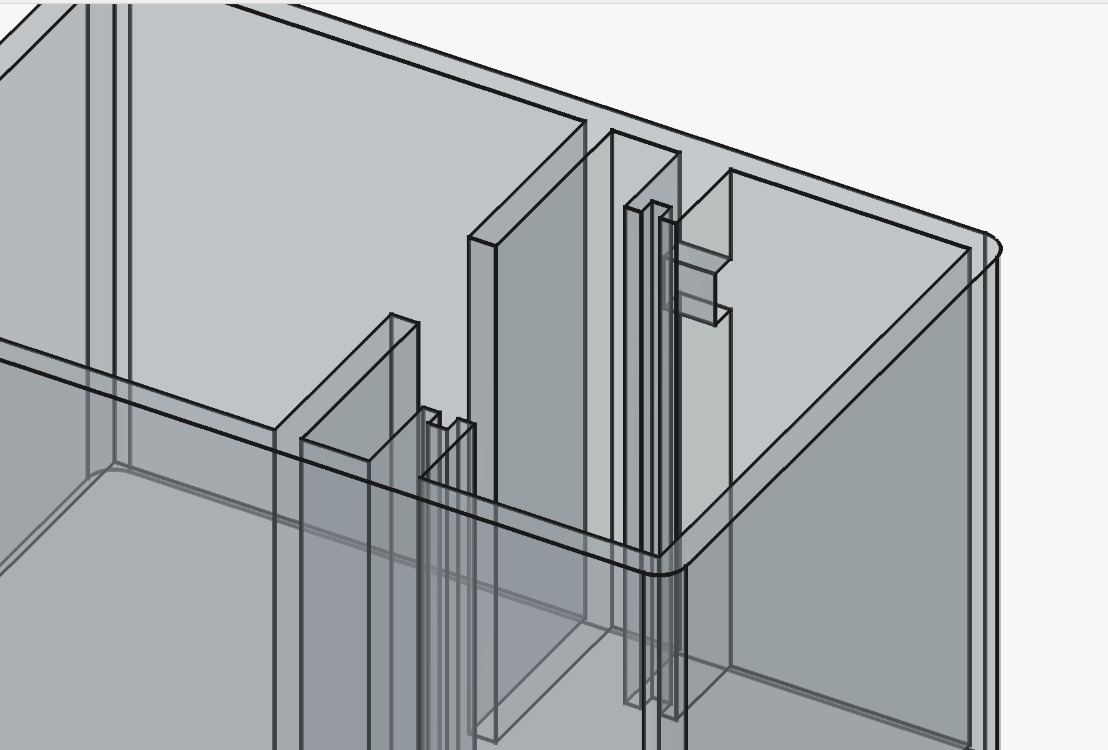
\includegraphics[width=\textwidth, height=11cm, keepaspectratio]{figs/CAD_7.jpeg}
\end{figure}
\noindent{This ended this day's work}
\section*{Day 8}
\noindent{We proceeded with making the compartment for the USB port. This was how it looked:}
\begin{figure}[H]
\centering
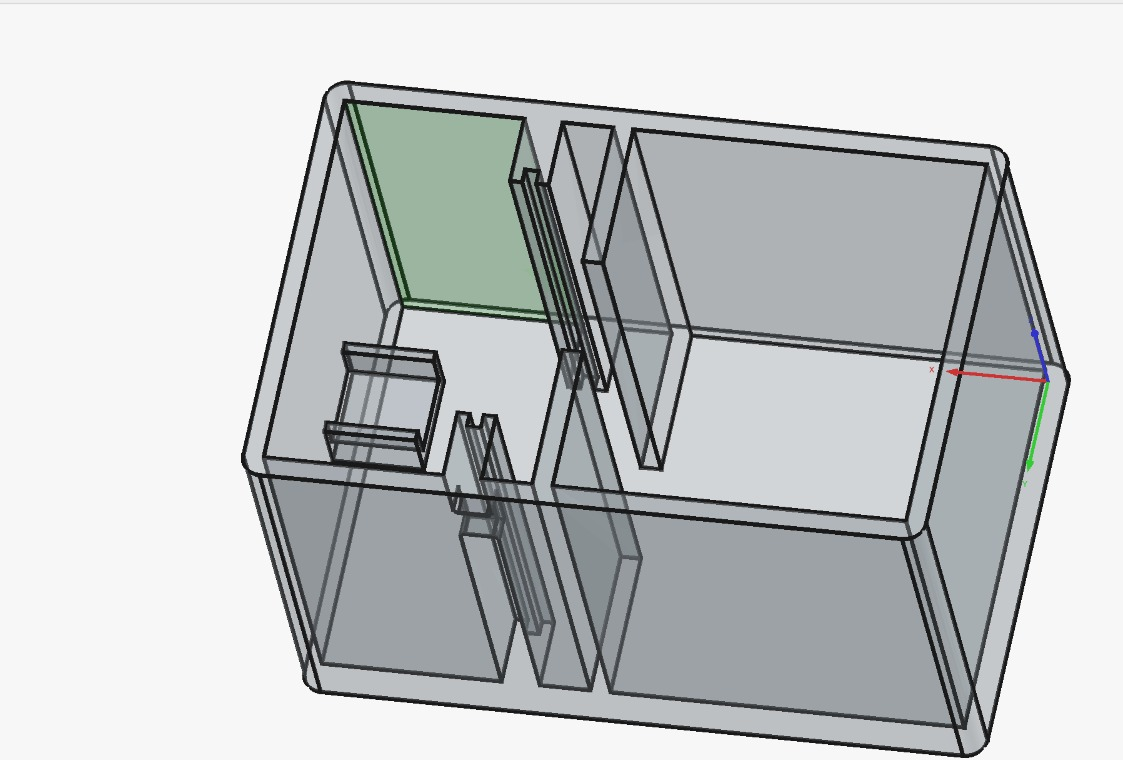
\includegraphics[width=\textwidth, height=11cm, keepaspectratio]{figs/CAD_8.jpeg}
\end{figure}

\noindent{Now, we added a stop at the back for the USB, just for extra support}
\begin{figure}[H]
\centering
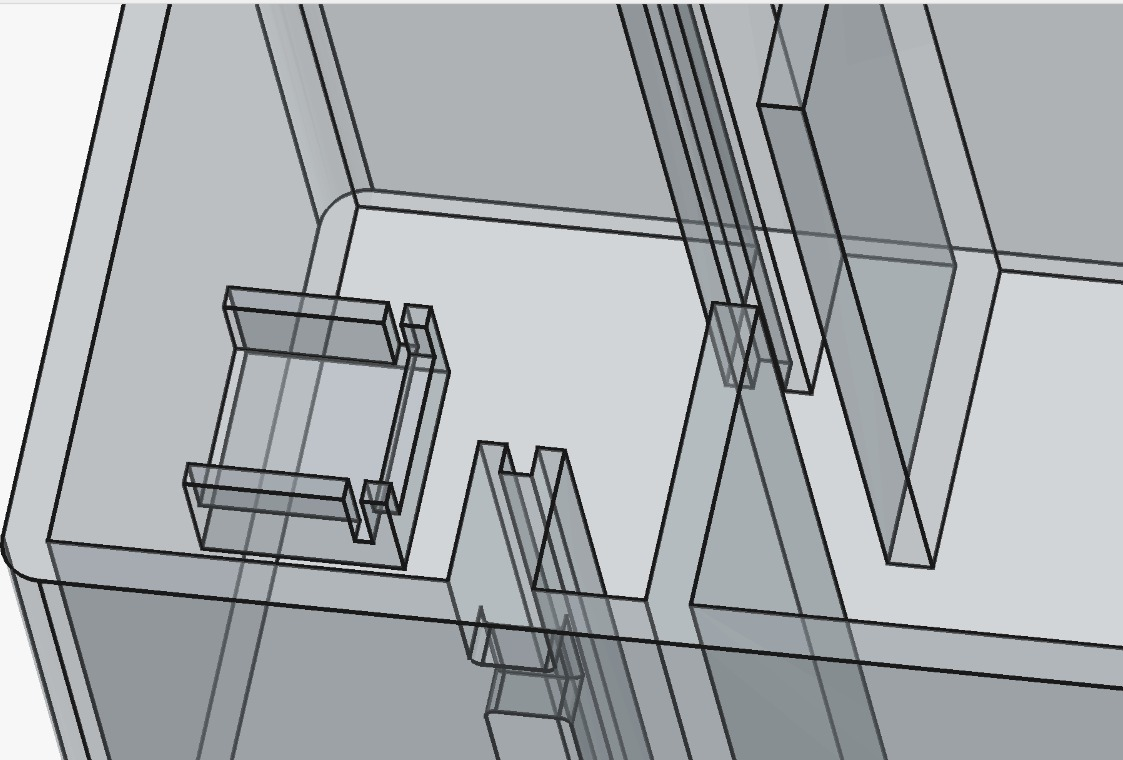
\includegraphics[width=\textwidth, height=11cm, keepaspectratio]{figs/CAD_9.jpeg}
\end{figure}
\noindent{We made the pocket for the USB next. The next step was to add the sliding mechanism somehow, and we were unsure of how to proceed, however we just began by making the grooves/rails for the lid to slide, as seen in the figure below.}
\begin{figure}[H]
\centering
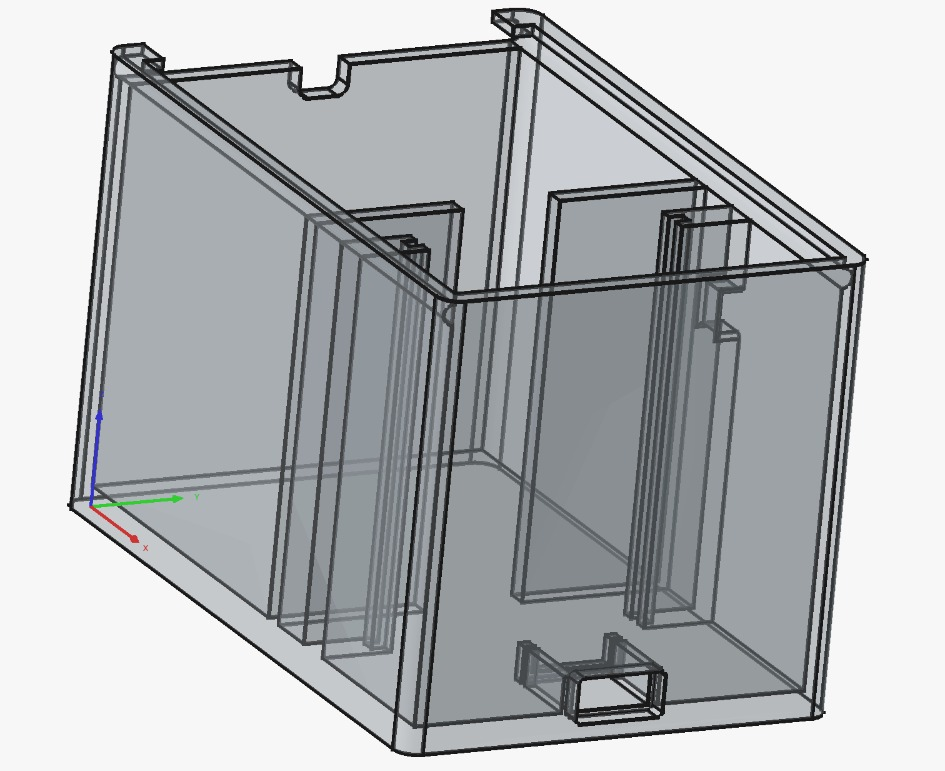
\includegraphics[width=\textwidth, height=11cm, keepaspectratio]{figs/CAD_11.jpeg}
\end{figure}
\noindent{We then created a sliding lid and made a depression in middle for opening/closing . We further added two holes for pegs to be inserted. Here the idea was that the pegs will stop the lid from sliding out.}
\begin{figure}[H]
    \centering

    \begin{subfigure}{0.45\textwidth}
    \centering
        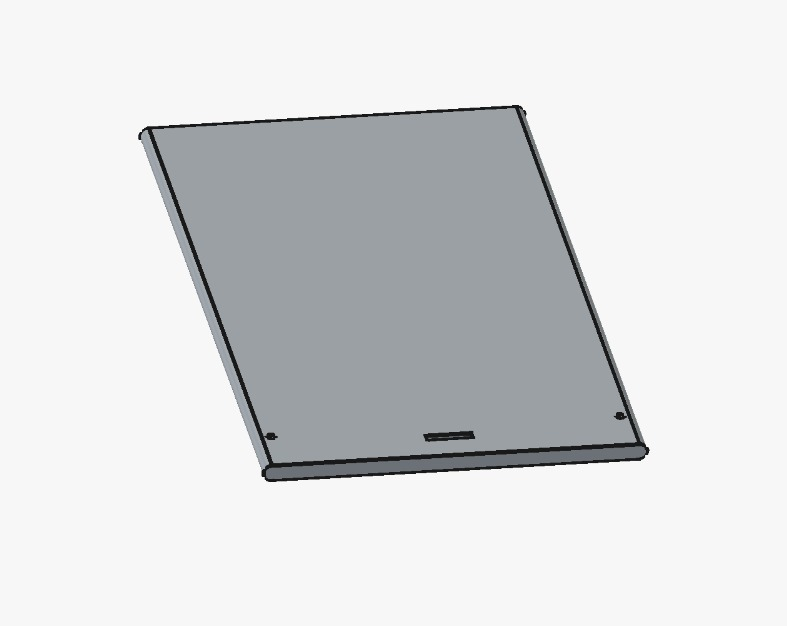
\includegraphics[width=\textwidth, height=10cm, keepaspectratio]{figs/CAD_12.jpeg}
        \caption{Lid}
    \end{subfigure}
    \hfill
    \begin{subfigure}{0.45\textwidth}
    \centering
        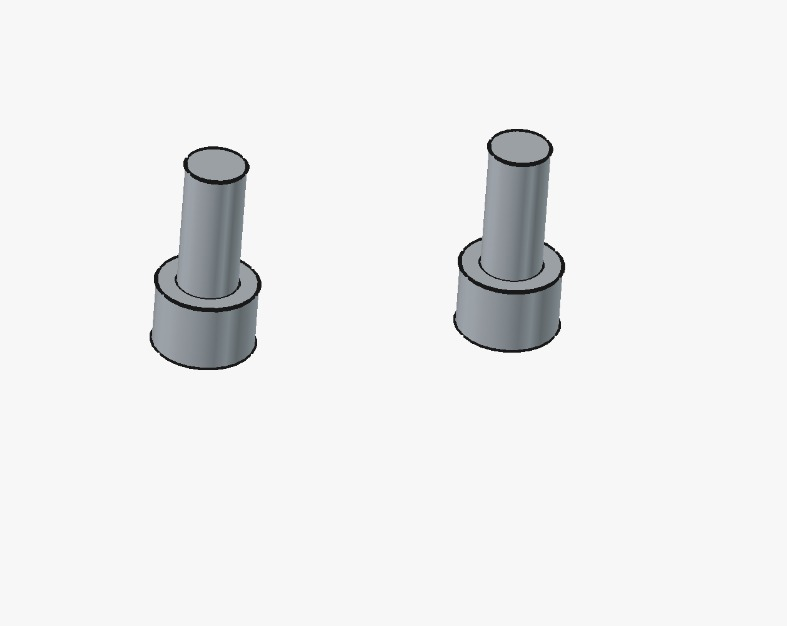
\includegraphics[width=\textwidth, height=9cm, keepaspectratio]{figs/CAD_13.jpeg}
        \caption{Pegs}
    \end{subfigure}
\end{figure}
\noindent{However, upon discussing with seniors  we realised that going with the sliding option is not a great idea, as it is very easy to go wrong with the dimensions of the lid and tolerances are pretty hard to manage without having prior experiences with the printer and its settings. And also we realised that if we were going to add pegs, it wouldn't be a permanent solution, and if were going to add pegs anyways, we might as well remove the sliding mechanism and just use screws for the lid.} 
\section*{Day 9}
\noindent{Before switching over from the sliding idea to screws, we added the supports for the transformer to prevent horizontal movement.}
\begin{figure}[H]
\centering
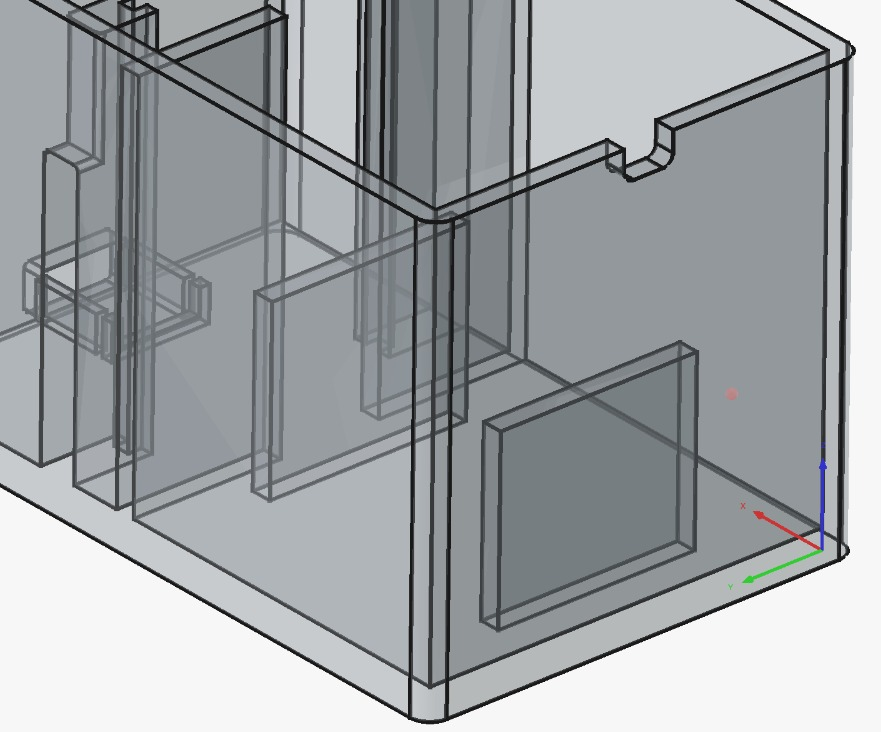
\includegraphics[width=\textwidth, height=11cm, keepaspectratio]{figs/CAD_17.jpeg}
\end{figure}
\noindent{Now, we added screw holes on top of the case}
\begin{figure}[H]
\centering
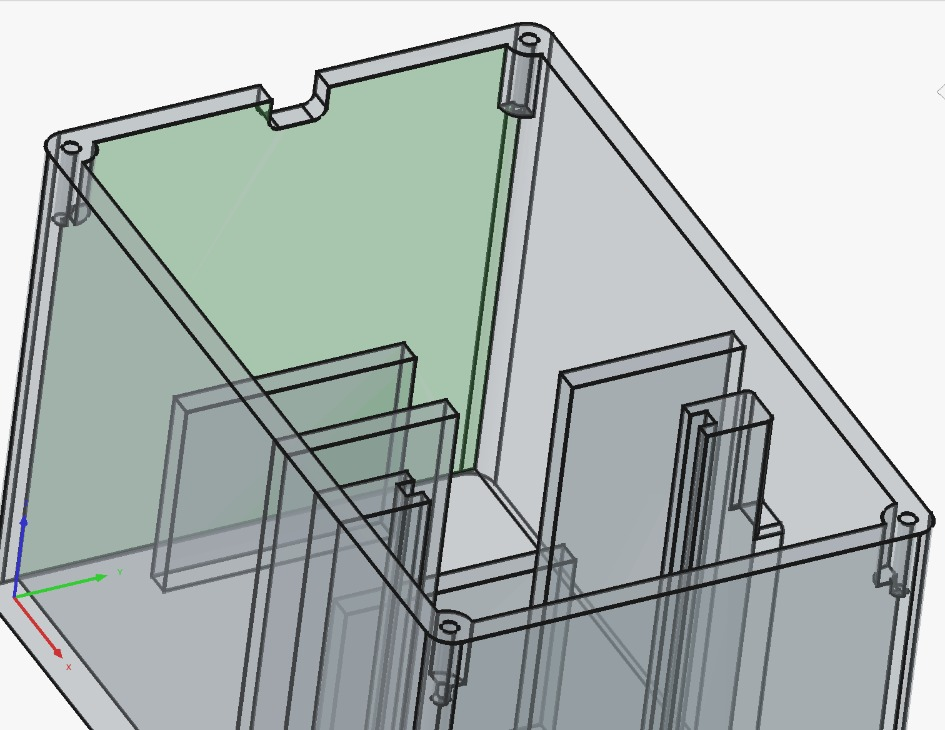
\includegraphics[width=\textwidth, height=11cm, keepaspectratio]{figs/CAD_14.jpeg}
\end{figure}
\noindent{We had to also create a new lid, and make the screw holes for it as well. We designed all screw holes considering M3 screws and adding appropriate tolerance.}
\begin{figure}[H]
    \centering

    \begin{subfigure}{0.45\textwidth}
    \centering
        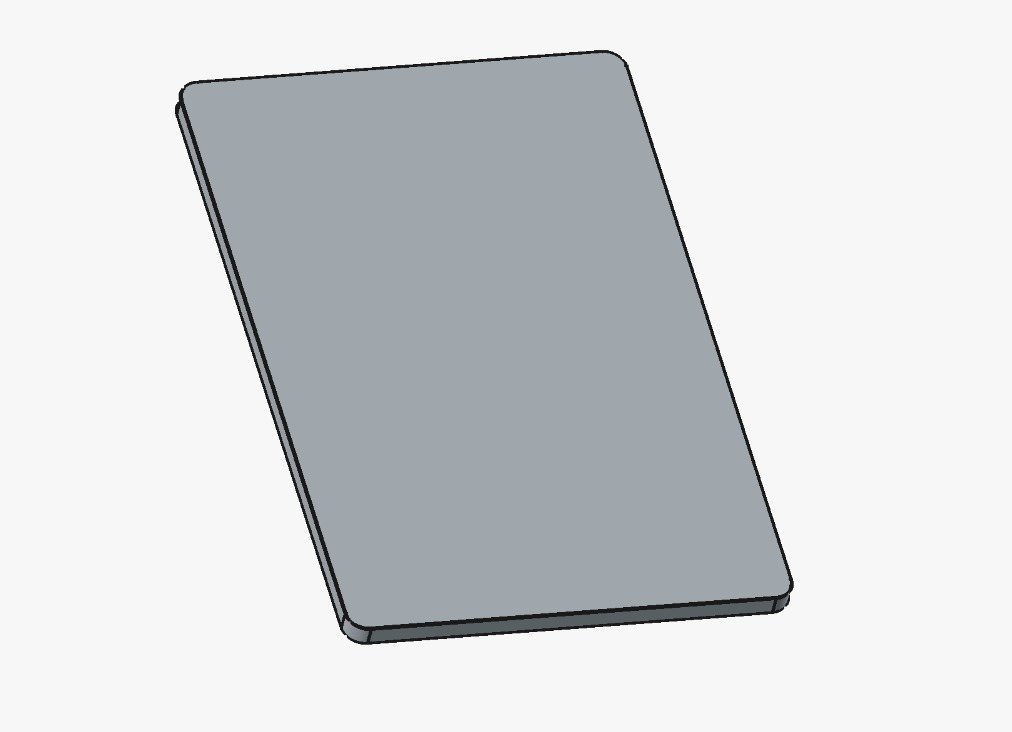
\includegraphics[width=\textwidth, height=10cm, keepaspectratio]{figs/CAD_15.jpeg}
        \caption{Lid}
    \end{subfigure}
    \hfill
    \begin{subfigure}{0.45\textwidth}
    \centering
        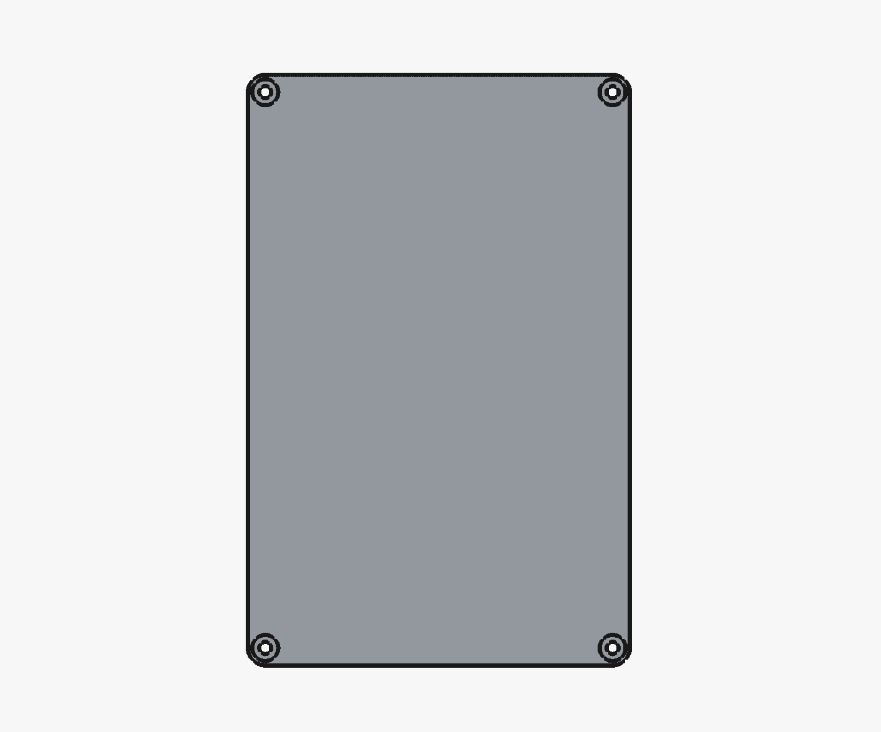
\includegraphics[width=\textwidth, height=9cm, keepaspectratio]{figs/CAD_16.jpeg}
        \caption{Adding screw holes}
    \end{subfigure}
\end{figure}
\noindent{We were done with the major part of the model now. Another thing that became easier now that we removed the sliding mechanism was the vertical support for the transformer, as it shouldn't oscillate when the case is rotated. So, we added a support on the lid to stop vertical displacement of transformer and filleted it, as shown in the following figure:}
\begin{figure}[H]
\centering
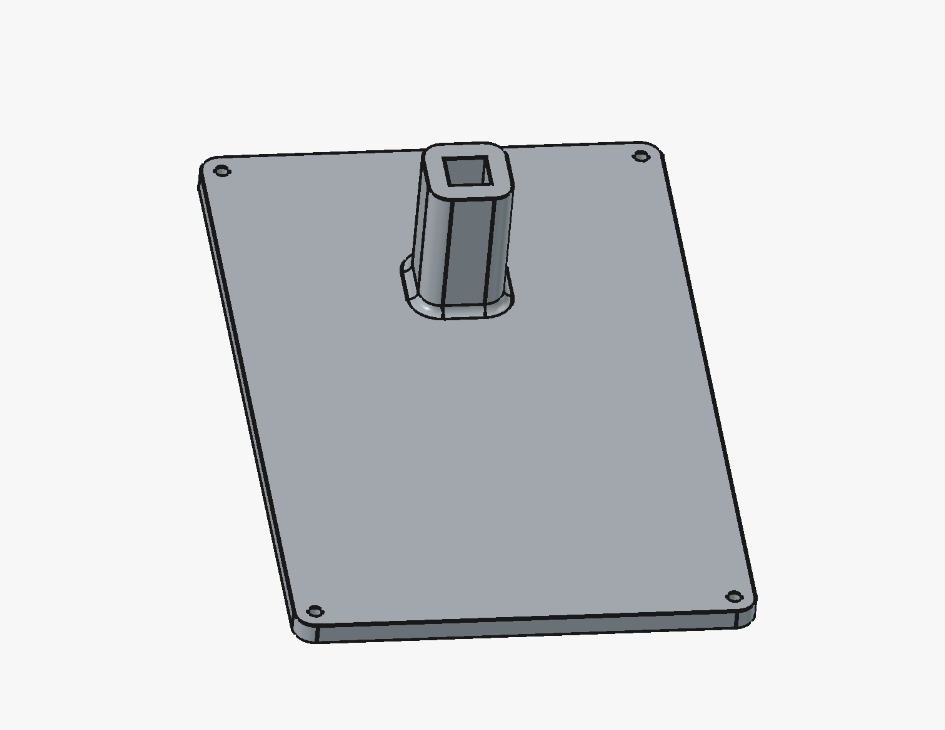
\includegraphics[width=\textwidth, height=11cm, keepaspectratio]{figs/CAD_18.jpeg}
\end{figure}
\noindent{Another thing we noticed was that the regulator's heat sink got quite hot upon use. Hence we decided to add perforations on the case and on the lid for ventilation.}
\begin{figure}[H]
\centering
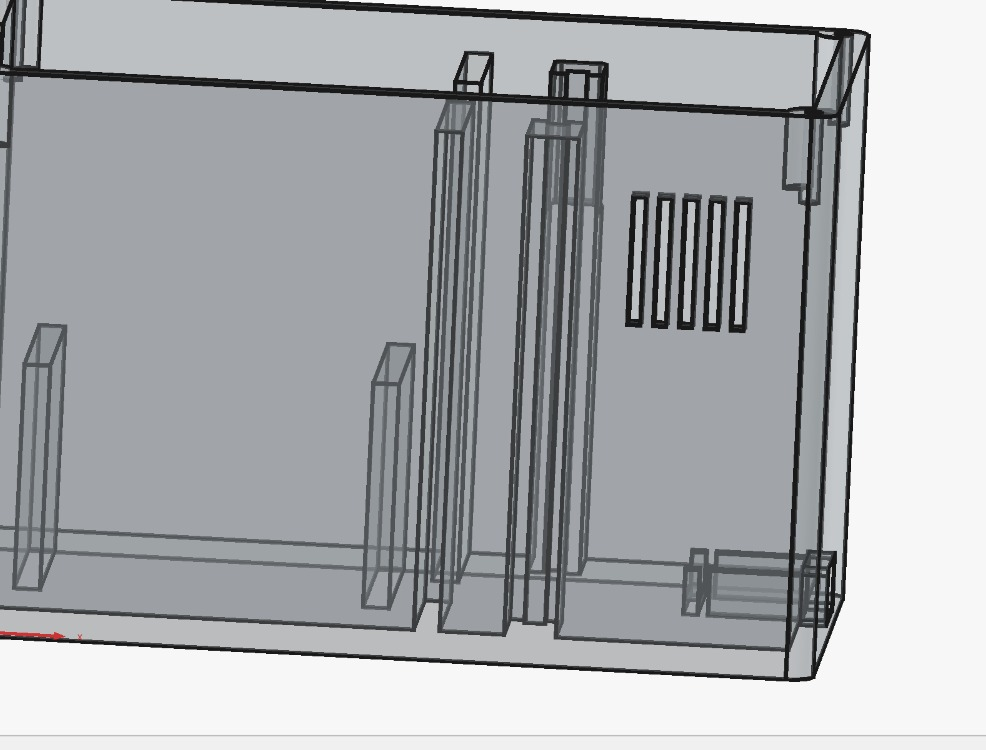
\includegraphics[width=\textwidth, height=11cm, keepaspectratio]{figs/CAD_19.jpeg}
\end{figure}
\begin{figure}[H]
\centering
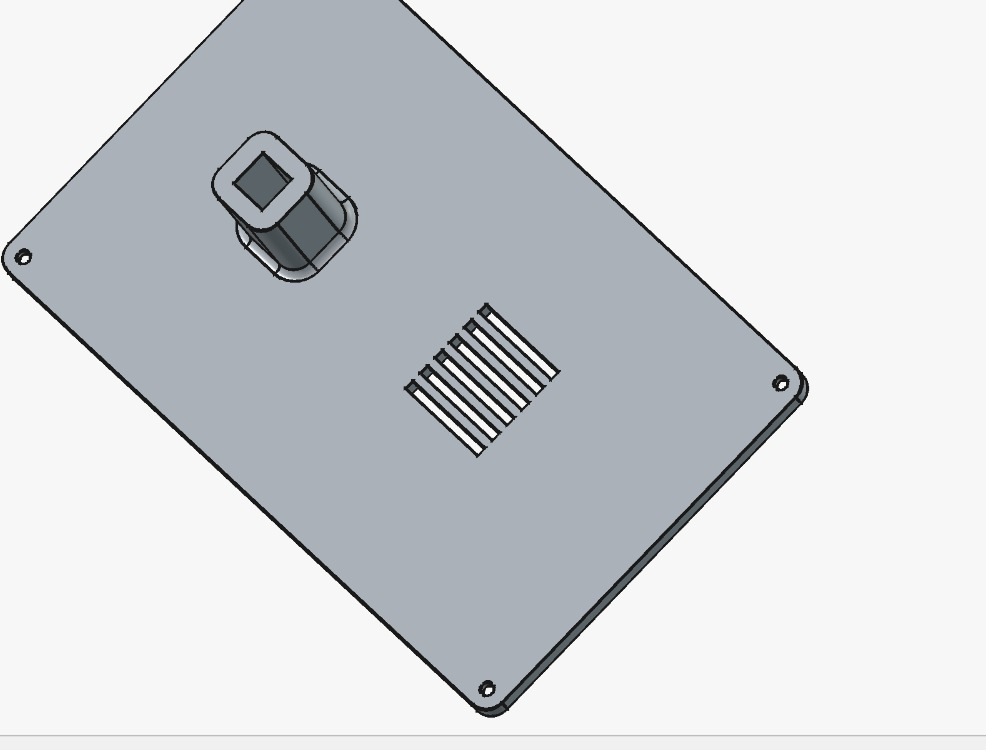
\includegraphics[width=\textwidth, height=11cm, keepaspectratio]{figs/CAD_20.jpeg}
\end{figure}
\clearpage
\section*{Day 10}
\noindent{Now that we finished designing the basic circuit, we wanted to add a few changes to the filter, as we got to know about the extension of the deadline for submission of the project. The current circuit utilises a $100 \mu F$ capacitor as a low pass filter. Upon researching, we found that this was not the best method to incorporate a filter into the circuit. This was the most basic method and we wanted to improve the filter. Having a better filter reduces the load on the regulator: The regulator itself has ripple rejection, meaning it reduces changes in its input voltage. Improving the filter will therefore make sure that the regulator is dealing with a smaller variation.}
\\ \\
\noindent{These were the methods we found:}
\begin{itemize}
    \item Using two capacitors
    \item Using two capacitors and a resistor
    \item Using two capacitors and an inductor
\end{itemize}
\noindent{We decided to avoid using the resistor as it would produce heat, further adding onto the heat produced by the regulator. Now we had to choose if we wanted to add an inductor or not. While not helping in smoothening the voltage, the inductor helps in smoothening the current, further improving the filter. Hence, we decided to add it.This was the circuit diagram for the filter:}
\begin{figure}[H]
    \centering
    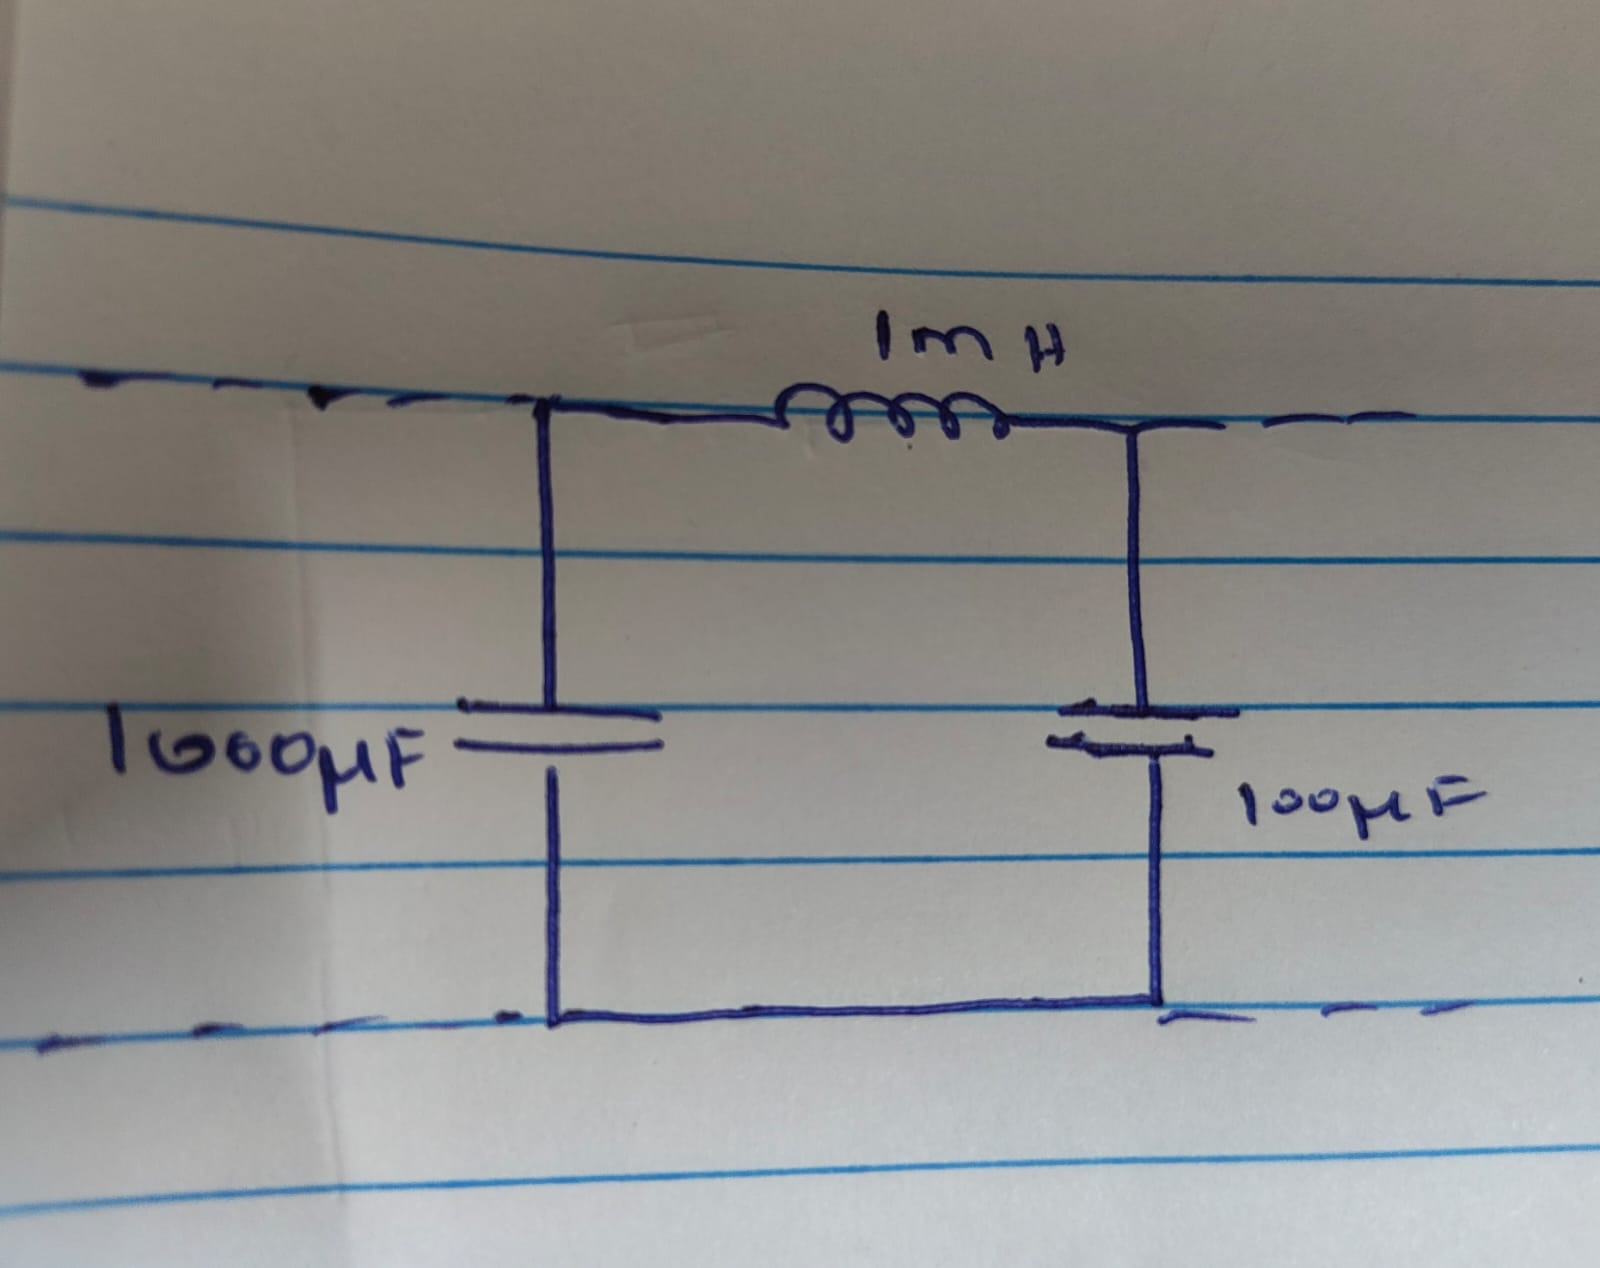
\includegraphics[width=\textwidth, height=10cm, keepaspectratio]{figs/filter_circuit.jpeg}
\end{figure}
\noindent{We then designed the circuit on the breadboard. We measured the voltage across the regulator and took the oscilloscope readings. We found that the ripple was very small between $1.2mV$ and $2.4mV$.}
\begin{figure}[H]
    \centering
    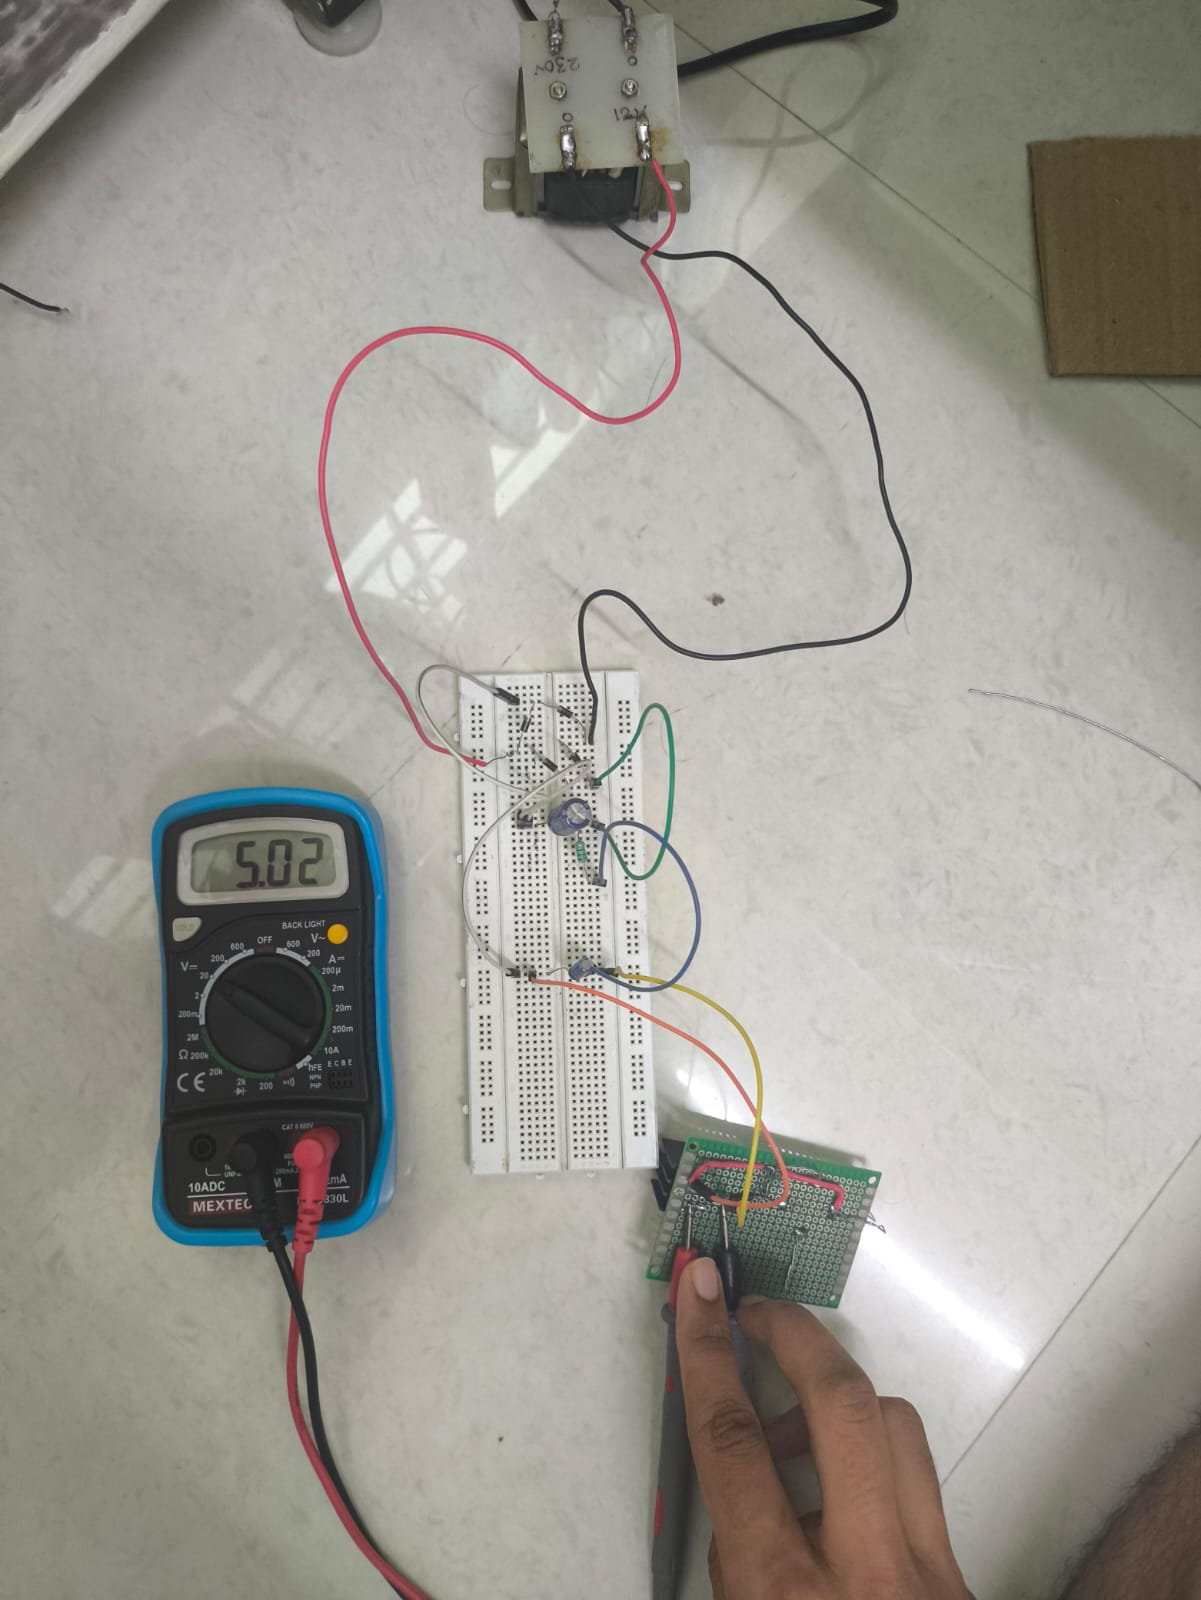
\includegraphics[width=\textwidth, height=10cm, keepaspectratio]{figs/Multimeter_changing_filter.jpeg}

\end{figure}
\begin{figure}[H]
    \centering
    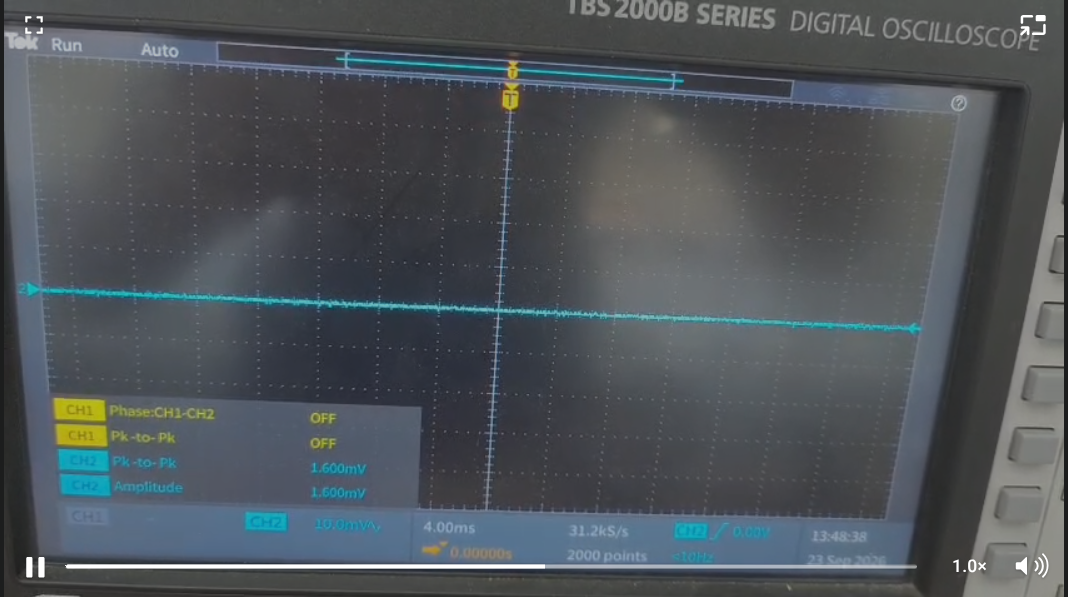
\includegraphics[width=\textwidth, height=10cm, keepaspectratio]{figs/Oscilloscope.png}

\end{figure}
\noindent{We finished the circuit by soldering the remaining two transformer wires onto the perfboard, cutting a few wires and cleaning up the solders.}
\noindent{With this setup, the power the phone was receiving was around $1W$. We wanted to try and increase this power as well. Upon researching, the easiest thing we found to increase the power was shorting the data pins. However, this only increased the power to around $2W$. This was because the 7805 regulator didn't allow the current delivered to go above a certain threshold. \\ \\
\noindent{This was the final circuit}
\begin{figure}[H]
    \centering

    \begin{subfigure}[H]{0.45\textwidth}
    \centering
        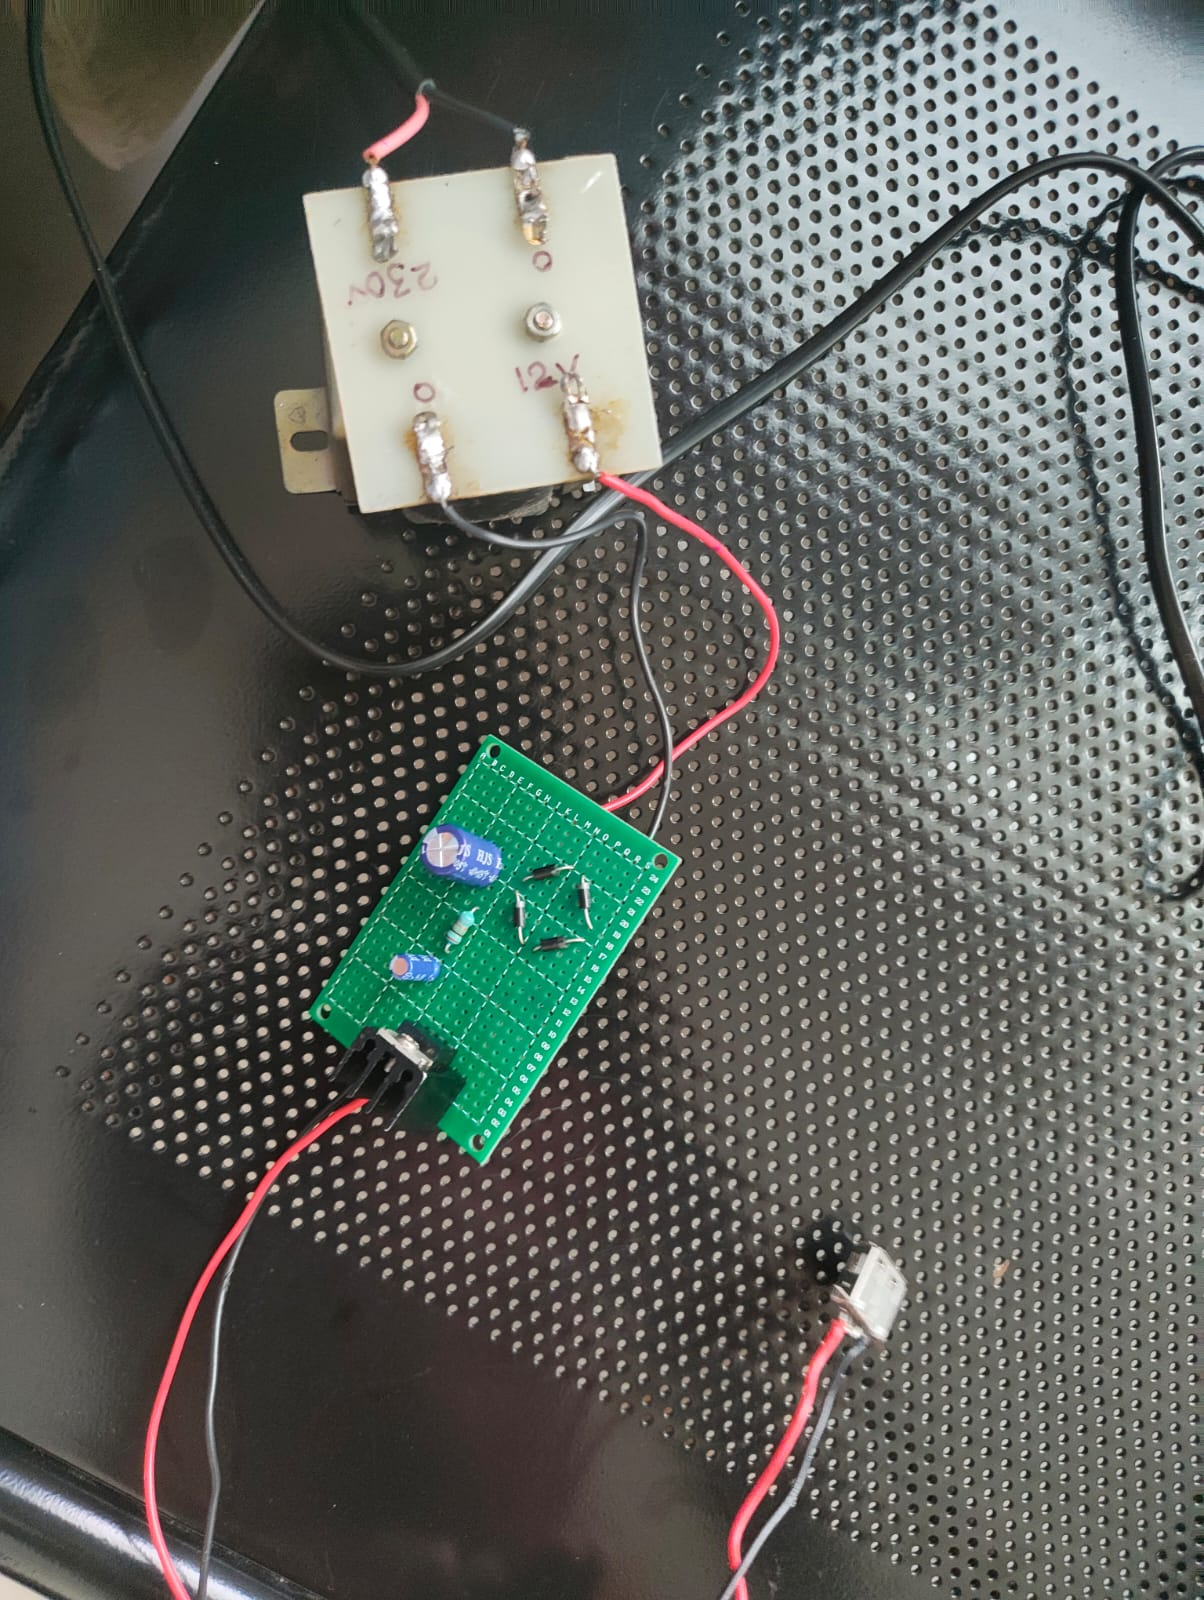
\includegraphics[width=\textwidth, height=8cm, keepaspectratio]{figs/Final_circuit_1.jpeg}
        \caption{Circuit}
    \end{subfigure}
    \hfill
    \begin{subfigure}[H]{0.45\textwidth}
    \centering
        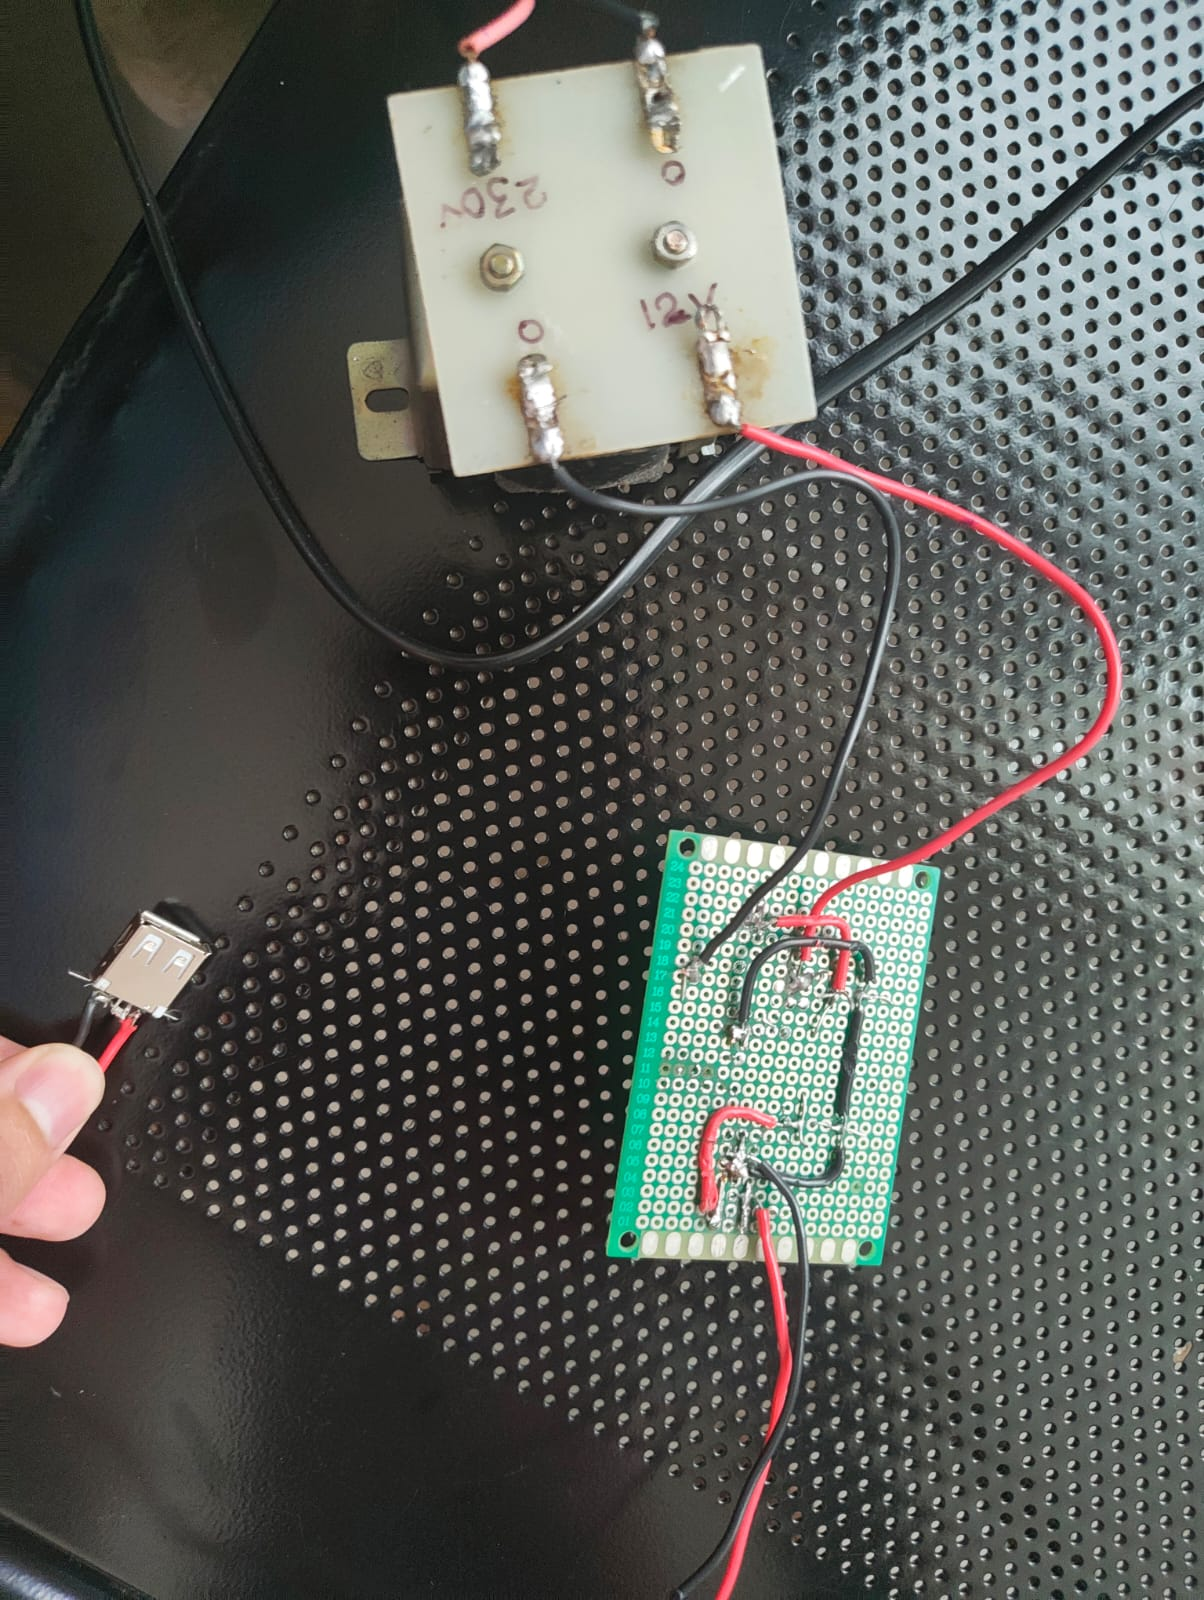
\includegraphics[width=\textwidth, height=8cm, keepaspectratio]{figs/Final_circuit_2.jpeg}
        \caption{Soldering}
    \end{subfigure}


\end{figure}
\section*{Future Work}
\noindent{We want to add the buck converter to the circuit in order to increase the efficiency and the power output. Depending on the results we get, we would like to further explore and research about ideas to increase the power output. We would also like to explore adding protection for current values that are too high.}
\section*{Learnings}
\begin{itemize}
\item Got an idea of soldering, and as the project progressed we became better at soldering, and de-soldering. We realised was that the best way to solder was to heat the pad and component together, and then feed solder int o the heated joint. Another thing we learnt was to avoid use of excess solder in case of a mess-up, and rather melt the available solder and reshape it.
\item Gained hands-on experience using multimeters and digital oscilloscopes to verify stage-by-stage outputs, voltage regulation (achieving an expected 5.02V output), and ripple voltage amplitudes.
\item Learned basic parametric CAD modeling techniques in FreeCAD
\item Learnt more about time management and planning - We felt that if we had planned the project better, we could have added more changes and implemented components like the buck converter etc.
\item Learnt about working in a team better, and sitting and brainstorming for ideas, when both of us were clueless about how to proceed, and learning from each other's thought processes. 
\end{itemize}
\end{document}


